\documentclass[aspectratio=169,11pt]{beamer}
% ==========================================================================
%  KSA lecture-slide theme  =  stock beamer "Boadilla"  +  KSA colour theme
%  brand colours sampled from the official KSA symbol mark:
%    Deep Prussian Blue  #2E3192   (지성 - intellect)
%    Golden Gray         #D6CBB1   (감성 - sensibility)
%  Engine: XeLaTeX.  Usage:
%    \documentclass[aspectratio=169,11pt]{beamer}
%    % ==========================================================================
%  KSA lecture-slide theme  =  stock beamer "Boadilla"  +  KSA colour theme
%  brand colours sampled from the official KSA symbol mark:
%    Deep Prussian Blue  #2E3192   (지성 - intellect)
%    Golden Gray         #D6CBB1   (감성 - sensibility)
%  Engine: XeLaTeX.  Usage:
%    \documentclass[aspectratio=169,11pt]{beamer}
%    % ==========================================================================
%  KSA lecture-slide theme  =  stock beamer "Boadilla"  +  KSA colour theme
%  brand colours sampled from the official KSA symbol mark:
%    Deep Prussian Blue  #2E3192   (지성 - intellect)
%    Golden Gray         #D6CBB1   (감성 - sensibility)
%  Engine: XeLaTeX.  Usage:
%    \documentclass[aspectratio=169,11pt]{beamer}
%    \input{../theme/ksa-theme.tex}
% ==========================================================================

\usepackage{fontspec}
\usepackage{amsmath,amssymb}
\usepackage{graphicx}
\graphicspath{{figs/}{../figs/}}
\usepackage{booktabs}
\usepackage{listings}

% ---- fonts (no ctex/xeCJK on this box -> fontspec drives CJK directly) -----
\defaultfontfeatures{Ligatures=TeX}
\setmainfont{Noto Sans CJK KR}
\setsansfont{Noto Sans CJK KR}
\setmonofont{Noto Sans Mono CJK KR}[Scale=0.92]

% ---- base theme: stock Boadilla ------------------------------------------
\usetheme{Boadilla}
\usefonttheme{professionalfonts}
\setbeamertemplate{navigation symbols}{}

% ---- KSA colour theme (recolour the stock theme) --------------------------
\definecolor{ksablue}{HTML}{2E3192}
\definecolor{ksabluedk}{HTML}{20226A}
\definecolor{ksagold}{HTML}{D6CBB1}
\definecolor{ksagolddk}{HTML}{A9976B}
\definecolor{ksared}{HTML}{C0392B}
\definecolor{ksagray}{HTML}{5B5B5B}

\setbeamercolor{structure}{fg=ksablue}
\setbeamercolor{alerted text}{fg=ksared}

\setbeamercolor{palette primary}{fg=white,           bg=ksablue}
\setbeamercolor{palette secondary}{fg=white,         bg=ksablue!85!black}
\setbeamercolor{palette tertiary}{fg=white,          bg=ksabluedk}
\setbeamercolor{titlelike}{fg=ksablue}
\setbeamercolor{frametitle}{fg=ksablue,bg=}
\setbeamercolor{title}{fg=ksablue}
\setbeamercolor{author}{fg=ksagray}
\setbeamercolor{institute}{fg=ksagray}
\setbeamercolor{block title}{fg=white,bg=ksablue}
\setbeamercolor{block body}{fg=black!85,bg=ksablue!6}
\setbeamercolor{item}{fg=ksablue}
\setbeamercolor{section in toc}{fg=black!85}

\setbeamerfont{frametitle}{series=\bfseries}
\setbeamerfont{title}{series=\bfseries}

% ---- footline:  KSA mark | "Made by ..." | n / N   (matches reference) ----
\newcommand{\ksacredit}{Made by Sumin Han \,\textperiodcentered\, suminhan@ksa.hs.kr}
\setbeamertemplate{footline}{%
  \hbox{%
    \begin{beamercolorbox}[wd=.18\paperwidth,ht=2.6ex,dp=1.5ex,leftskip=1.1em]{}%
      \raisebox{-0.35ex}{
\includegraphics[height=2.0ex]{ksa-logo.png}}%
    \end{beamercolorbox}%
    \begin{beamercolorbox}[wd=.64\paperwidth,ht=2.6ex,dp=1.5ex,center]{}%
      {\scriptsize\color{ksagray}\ksacredit}%
    \end{beamercolorbox}%
    \begin{beamercolorbox}[wd=.18\paperwidth,ht=2.6ex,dp=1.5ex,rightskip=1.1em]{}%
      \hfill{\scriptsize\color{ksablue}\insertframenumber\,/\,\inserttotalframenumber}%
    \end{beamercolorbox}%
  }%
  \vskip2pt
}

% ---- section divider: stock \sectionpage, KSA-coloured -------------------
\setbeamertemplate{section page}{%
  \begingroup\centering
    {\color{ksagolddk}\rule{0.16\paperwidth}{1pt}}\par\vskip1.0em
    {\usebeamerfont{title}\color{ksablue}\insertsectionhead\par}\vskip1.0em
    {\color{ksagolddk}\rule{0.16\paperwidth}{1pt}}\par
  \endgroup
}
\AtBeginSection[]{\begin{frame}[plain,noframenumbering]\vfill\sectionpage\vfill\end{frame}}

% ---- code listings ------------------------------------------------------------
\lstdefinestyle{ksa}{%
  basicstyle=\ttfamily\scriptsize,
  keywordstyle=\color{ksablue}\bfseries,
  commentstyle=\color{ksagray}\itshape,
  stringstyle=\color{ksagolddk},
  numberstyle=\tiny\color{ksagray},
  backgroundcolor=\color{ksablue!6},
  frame=leftline, framerule=1.4pt, rulecolor=\color{ksablue},
  xleftmargin=1em, aboveskip=0.8em, belowskip=0.4em,
  showstringspaces=false, breaklines=true, language=Python,
}
\lstset{style=ksa}

% ---- handy macros -----------------------------------------------------------
\newcommand{\kb}[1]{\textbf{\color{ksablue}#1}}   % blue keyword
\newcommand{\kq}[1]{\textbf{\color{ksared}#1}}    % red key-question

% ==========================================================================

\usepackage{fontspec}
\usepackage{amsmath,amssymb}
\usepackage{graphicx}
\graphicspath{{figs/}{../figs/}}
\usepackage{booktabs}
\usepackage{listings}

% ---- fonts (no ctex/xeCJK on this box -> fontspec drives CJK directly) -----
\defaultfontfeatures{Ligatures=TeX}
\setmainfont{Noto Sans CJK KR}
\setsansfont{Noto Sans CJK KR}
\setmonofont{Noto Sans Mono CJK KR}[Scale=0.92]

% ---- base theme: stock Boadilla ------------------------------------------
\usetheme{Boadilla}
\usefonttheme{professionalfonts}
\setbeamertemplate{navigation symbols}{}

% ---- KSA colour theme (recolour the stock theme) --------------------------
\definecolor{ksablue}{HTML}{2E3192}
\definecolor{ksabluedk}{HTML}{20226A}
\definecolor{ksagold}{HTML}{D6CBB1}
\definecolor{ksagolddk}{HTML}{A9976B}
\definecolor{ksared}{HTML}{C0392B}
\definecolor{ksagray}{HTML}{5B5B5B}

\setbeamercolor{structure}{fg=ksablue}
\setbeamercolor{alerted text}{fg=ksared}

\setbeamercolor{palette primary}{fg=white,           bg=ksablue}
\setbeamercolor{palette secondary}{fg=white,         bg=ksablue!85!black}
\setbeamercolor{palette tertiary}{fg=white,          bg=ksabluedk}
\setbeamercolor{titlelike}{fg=ksablue}
\setbeamercolor{frametitle}{fg=ksablue,bg=}
\setbeamercolor{title}{fg=ksablue}
\setbeamercolor{author}{fg=ksagray}
\setbeamercolor{institute}{fg=ksagray}
\setbeamercolor{block title}{fg=white,bg=ksablue}
\setbeamercolor{block body}{fg=black!85,bg=ksablue!6}
\setbeamercolor{item}{fg=ksablue}
\setbeamercolor{section in toc}{fg=black!85}

\setbeamerfont{frametitle}{series=\bfseries}
\setbeamerfont{title}{series=\bfseries}

% ---- footline:  KSA mark | "Made by ..." | n / N   (matches reference) ----
\newcommand{\ksacredit}{Made by Sumin Han \,\textperiodcentered\, suminhan@ksa.hs.kr}
\setbeamertemplate{footline}{%
  \hbox{%
    \begin{beamercolorbox}[wd=.18\paperwidth,ht=2.6ex,dp=1.5ex,leftskip=1.1em]{}%
      \raisebox{-0.35ex}{
\includegraphics[height=2.0ex]{ksa-logo.png}}%
    \end{beamercolorbox}%
    \begin{beamercolorbox}[wd=.64\paperwidth,ht=2.6ex,dp=1.5ex,center]{}%
      {\scriptsize\color{ksagray}\ksacredit}%
    \end{beamercolorbox}%
    \begin{beamercolorbox}[wd=.18\paperwidth,ht=2.6ex,dp=1.5ex,rightskip=1.1em]{}%
      \hfill{\scriptsize\color{ksablue}\insertframenumber\,/\,\inserttotalframenumber}%
    \end{beamercolorbox}%
  }%
  \vskip2pt
}

% ---- section divider: stock \sectionpage, KSA-coloured -------------------
\setbeamertemplate{section page}{%
  \begingroup\centering
    {\color{ksagolddk}\rule{0.16\paperwidth}{1pt}}\par\vskip1.0em
    {\usebeamerfont{title}\color{ksablue}\insertsectionhead\par}\vskip1.0em
    {\color{ksagolddk}\rule{0.16\paperwidth}{1pt}}\par
  \endgroup
}
\AtBeginSection[]{\begin{frame}[plain,noframenumbering]\vfill\sectionpage\vfill\end{frame}}

% ---- code listings ------------------------------------------------------------
\lstdefinestyle{ksa}{%
  basicstyle=\ttfamily\scriptsize,
  keywordstyle=\color{ksablue}\bfseries,
  commentstyle=\color{ksagray}\itshape,
  stringstyle=\color{ksagolddk},
  numberstyle=\tiny\color{ksagray},
  backgroundcolor=\color{ksablue!6},
  frame=leftline, framerule=1.4pt, rulecolor=\color{ksablue},
  xleftmargin=1em, aboveskip=0.8em, belowskip=0.4em,
  showstringspaces=false, breaklines=true, language=Python,
}
\lstset{style=ksa}

% ---- handy macros -----------------------------------------------------------
\newcommand{\kb}[1]{\textbf{\color{ksablue}#1}}   % blue keyword
\newcommand{\kq}[1]{\textbf{\color{ksared}#1}}    % red key-question

% ==========================================================================

\usepackage{fontspec}
\usepackage{amsmath,amssymb}
\usepackage{graphicx}
\graphicspath{{figs/}{../figs/}}
\usepackage{booktabs}
\usepackage{listings}

% ---- fonts (no ctex/xeCJK on this box -> fontspec drives CJK directly) -----
\defaultfontfeatures{Ligatures=TeX}
\setmainfont{Noto Sans CJK KR}
\setsansfont{Noto Sans CJK KR}
\setmonofont{Noto Sans Mono CJK KR}[Scale=0.92]

% ---- base theme: stock Boadilla ------------------------------------------
\usetheme{Boadilla}
\usefonttheme{professionalfonts}
\setbeamertemplate{navigation symbols}{}

% ---- KSA colour theme (recolour the stock theme) --------------------------
\definecolor{ksablue}{HTML}{2E3192}
\definecolor{ksabluedk}{HTML}{20226A}
\definecolor{ksagold}{HTML}{D6CBB1}
\definecolor{ksagolddk}{HTML}{A9976B}
\definecolor{ksared}{HTML}{C0392B}
\definecolor{ksagray}{HTML}{5B5B5B}

\setbeamercolor{structure}{fg=ksablue}
\setbeamercolor{alerted text}{fg=ksared}

\setbeamercolor{palette primary}{fg=white,           bg=ksablue}
\setbeamercolor{palette secondary}{fg=white,         bg=ksablue!85!black}
\setbeamercolor{palette tertiary}{fg=white,          bg=ksabluedk}
\setbeamercolor{titlelike}{fg=ksablue}
\setbeamercolor{frametitle}{fg=ksablue,bg=}
\setbeamercolor{title}{fg=ksablue}
\setbeamercolor{author}{fg=ksagray}
\setbeamercolor{institute}{fg=ksagray}
\setbeamercolor{block title}{fg=white,bg=ksablue}
\setbeamercolor{block body}{fg=black!85,bg=ksablue!6}
\setbeamercolor{item}{fg=ksablue}
\setbeamercolor{section in toc}{fg=black!85}

\setbeamerfont{frametitle}{series=\bfseries}
\setbeamerfont{title}{series=\bfseries}

% ---- footline:  KSA mark | "Made by ..." | n / N   (matches reference) ----
\newcommand{\ksacredit}{Made by Sumin Han \,\textperiodcentered\, suminhan@ksa.hs.kr}
\setbeamertemplate{footline}{%
  \hbox{%
    \begin{beamercolorbox}[wd=.18\paperwidth,ht=2.6ex,dp=1.5ex,leftskip=1.1em]{}%
      \raisebox{-0.35ex}{
\includegraphics[height=2.0ex]{ksa-logo.png}}%
    \end{beamercolorbox}%
    \begin{beamercolorbox}[wd=.64\paperwidth,ht=2.6ex,dp=1.5ex,center]{}%
      {\scriptsize\color{ksagray}\ksacredit}%
    \end{beamercolorbox}%
    \begin{beamercolorbox}[wd=.18\paperwidth,ht=2.6ex,dp=1.5ex,rightskip=1.1em]{}%
      \hfill{\scriptsize\color{ksablue}\insertframenumber\,/\,\inserttotalframenumber}%
    \end{beamercolorbox}%
  }%
  \vskip2pt
}

% ---- section divider: stock \sectionpage, KSA-coloured -------------------
\setbeamertemplate{section page}{%
  \begingroup\centering
    {\color{ksagolddk}\rule{0.16\paperwidth}{1pt}}\par\vskip1.0em
    {\usebeamerfont{title}\color{ksablue}\insertsectionhead\par}\vskip1.0em
    {\color{ksagolddk}\rule{0.16\paperwidth}{1pt}}\par
  \endgroup
}
\AtBeginSection[]{\begin{frame}[plain,noframenumbering]\vfill\sectionpage\vfill\end{frame}}

% ---- code listings ------------------------------------------------------------
\lstdefinestyle{ksa}{%
  basicstyle=\ttfamily\scriptsize,
  keywordstyle=\color{ksablue}\bfseries,
  commentstyle=\color{ksagray}\itshape,
  stringstyle=\color{ksagolddk},
  numberstyle=\tiny\color{ksagray},
  backgroundcolor=\color{ksablue!6},
  frame=leftline, framerule=1.4pt, rulecolor=\color{ksablue},
  xleftmargin=1em, aboveskip=0.8em, belowskip=0.4em,
  showstringspaces=false, breaklines=true, language=Python,
}
\lstset{style=ksa}

% ---- handy macros -----------------------------------------------------------
\newcommand{\kb}[1]{\textbf{\color{ksablue}#1}}   % blue keyword
\newcommand{\kq}[1]{\textbf{\color{ksared}#1}}    % red key-question


\title{머신러닝 첫걸음}
\subtitle{역사와 로드맵 \,\textperiodcentered\, 문제 정식화와 세 갈래 분류 \,\textperiodcentered\, 파이프라인과 사전지식 리뷰}
\author{Machine Learning 1 \,\textperiodcentered\, 1주차}
\institute{한국과학영재학교 (KSA)}
\date{Chapter 1}

\begin{document}
\begin{frame}[plain,noframenumbering]\titlepage\end{frame}

% ===== 이번 주차 개요 =====
\begin{frame}{이번 주차 개요}
  \small
  이 챕터를 마치면:
  \begin{itemize}
    \item 1943$\sim$2025 연표 위에서 1969년과 2012년을 가로지른 \textbf{두 ``AI
      겨울''}의 원인을 각 한 문장으로 설명.
    \item 문제를 입력 $x$ · 출력 $y$ · 가설 $h$ 로 \kb{정식화}하고,
      ``라벨이 있는가? 보상이 있는가?'' 두 질문만으로 \kb{세 갈래} 분류.
    \item 회귀 vs 분류를 \textbf{``같은 모델, 다른 출력''}(항등 링크 vs
      시그모이드)으로 설명하고, \textbf{``손실함수 $J$ 를 정의하고
      최소화한다''}는 뼈대를 이름으로 부름.
    \item 수집 $\to$ 정제 $\to$ EDA $\to$ 모델링 $\to$ 평가 파이프라인을
      끝까지 돌리고, 결측치·중복·이상치와 \textbf{데이터 누수}를 잡는 순서를
      지킴.
  \end{itemize}
  \vskip0.6em
  \begin{block}{세 차시 한 줄}
    \kb{1.1} 역사·로드맵 \quad \kb{1.2} 문제 정의와 세 갈래
    \quad \kb{1.3} 데이터 파이프라인 + 세 가지 수학
  \end{block}
\end{frame}

% =================================================================
\section{1.1 아주 짧은 역사와 이번 학기 로드맵}

\begin{frame}{이 두 과목이 다루는 질문}
  2012년 ImageNet 대회에서 \kb{AlexNet} 이 등장하기 전까지, ``이 사진에
  고양이가 있는가''를 알려주는 방법은 \textbf{사람이 직접 특징을 설계}하는
  것이었다 --- 가장자리 검출기, 색 히스토그램, 특정 모양의 필터를 손으로
  조합해 ``고양이스러움''을 수치로 정의하려 했다.
  \vskip0.6em
  AlexNet은 그런 손설계 없이, 수백만 장의 사진과 정답 라벨만 보고
  \textbf{스스로 무엇을 봐야 하는지 학습}해서 기존 방법들을 압도적인 차이로
  이겼다.
  \vskip1em
  \begin{center}
  \kq{정답이 있는 데이터로부터, 규칙을 사람이 짜는 대신\\
      기계가 데이터에서 직접 찾아내게 하려면 어떻게 해야 하는가?}
  \end{center}
\end{frame}

\begin{frame}{아주 짧은 역사 --- 퍼셉트론에서 LLM까지}
  \small
  \begin{itemize}
    \item 이번 학기에 배울 아이디어들이 \textbf{언제, 어떤 순서로} 등장했는지
      알면 ``왜 지금 이 순서로 배우는가''가 더 잘 보인다.
    \item 흥미로운 점: 역사가 직선으로 발전한 게 아니라
      \kb{침체기(``AI 겨울'')를 두 번이나 거쳤다}는 것.
  \end{itemize}
  \vskip0.6em
  \begin{tabular}{@{}ll@{}}
    \toprule
    연도 & 사건 \\
    \midrule
    1943 & 맥컬록-피터즈 신경원 모형 --- ``수학적으로 학습 가능한 뉴런''의 시작 \\
    1950s & 퍼셉트론(단층 신경망) 등장 \\
    1969 & 민스키·페퍼트(1969)의 XOR 한계 증명 $\to$ \textbf{첫 AI 겨울} (Ch.\,9) \\
    1986 & 역전파(Rumelhart·Hinton·Williams, 1986) 재발견 $\to$ 다층 학습 가능 \\
    1998 & LeCun의 CNN(LeNet), 손글씨 숫자 인식 성공 (Ch.\,10) \\
    2012 & AlexNet, ImageNet 압승 --- \textbf{딥러닝 시대의 시작} \\
    2013 & word2vec · VAE --- 표현학습·생성모델의 현대적 형태 (Ch.\,14, 15) \\
    2017 & Transformer(``Attention Is All You Need'') (Ch.\,12) \\
    2022 & ChatGPT --- 사전학습 + RLHF로 조정된 대규모 언어모델의 대중화 \\
    2025 & GPT-4o·Gemini·Claude 등 멀티모달 LLM이 스마트폰·워크스테이션에 내장 \\
    \bottomrule
  \end{tabular}
\end{frame}

\begin{frame}{연표를 ``연도 축'' 위에 그리면}
  \small
  \begin{columns}[T]
    \begin{column}{0.48\textwidth}
      \centering
      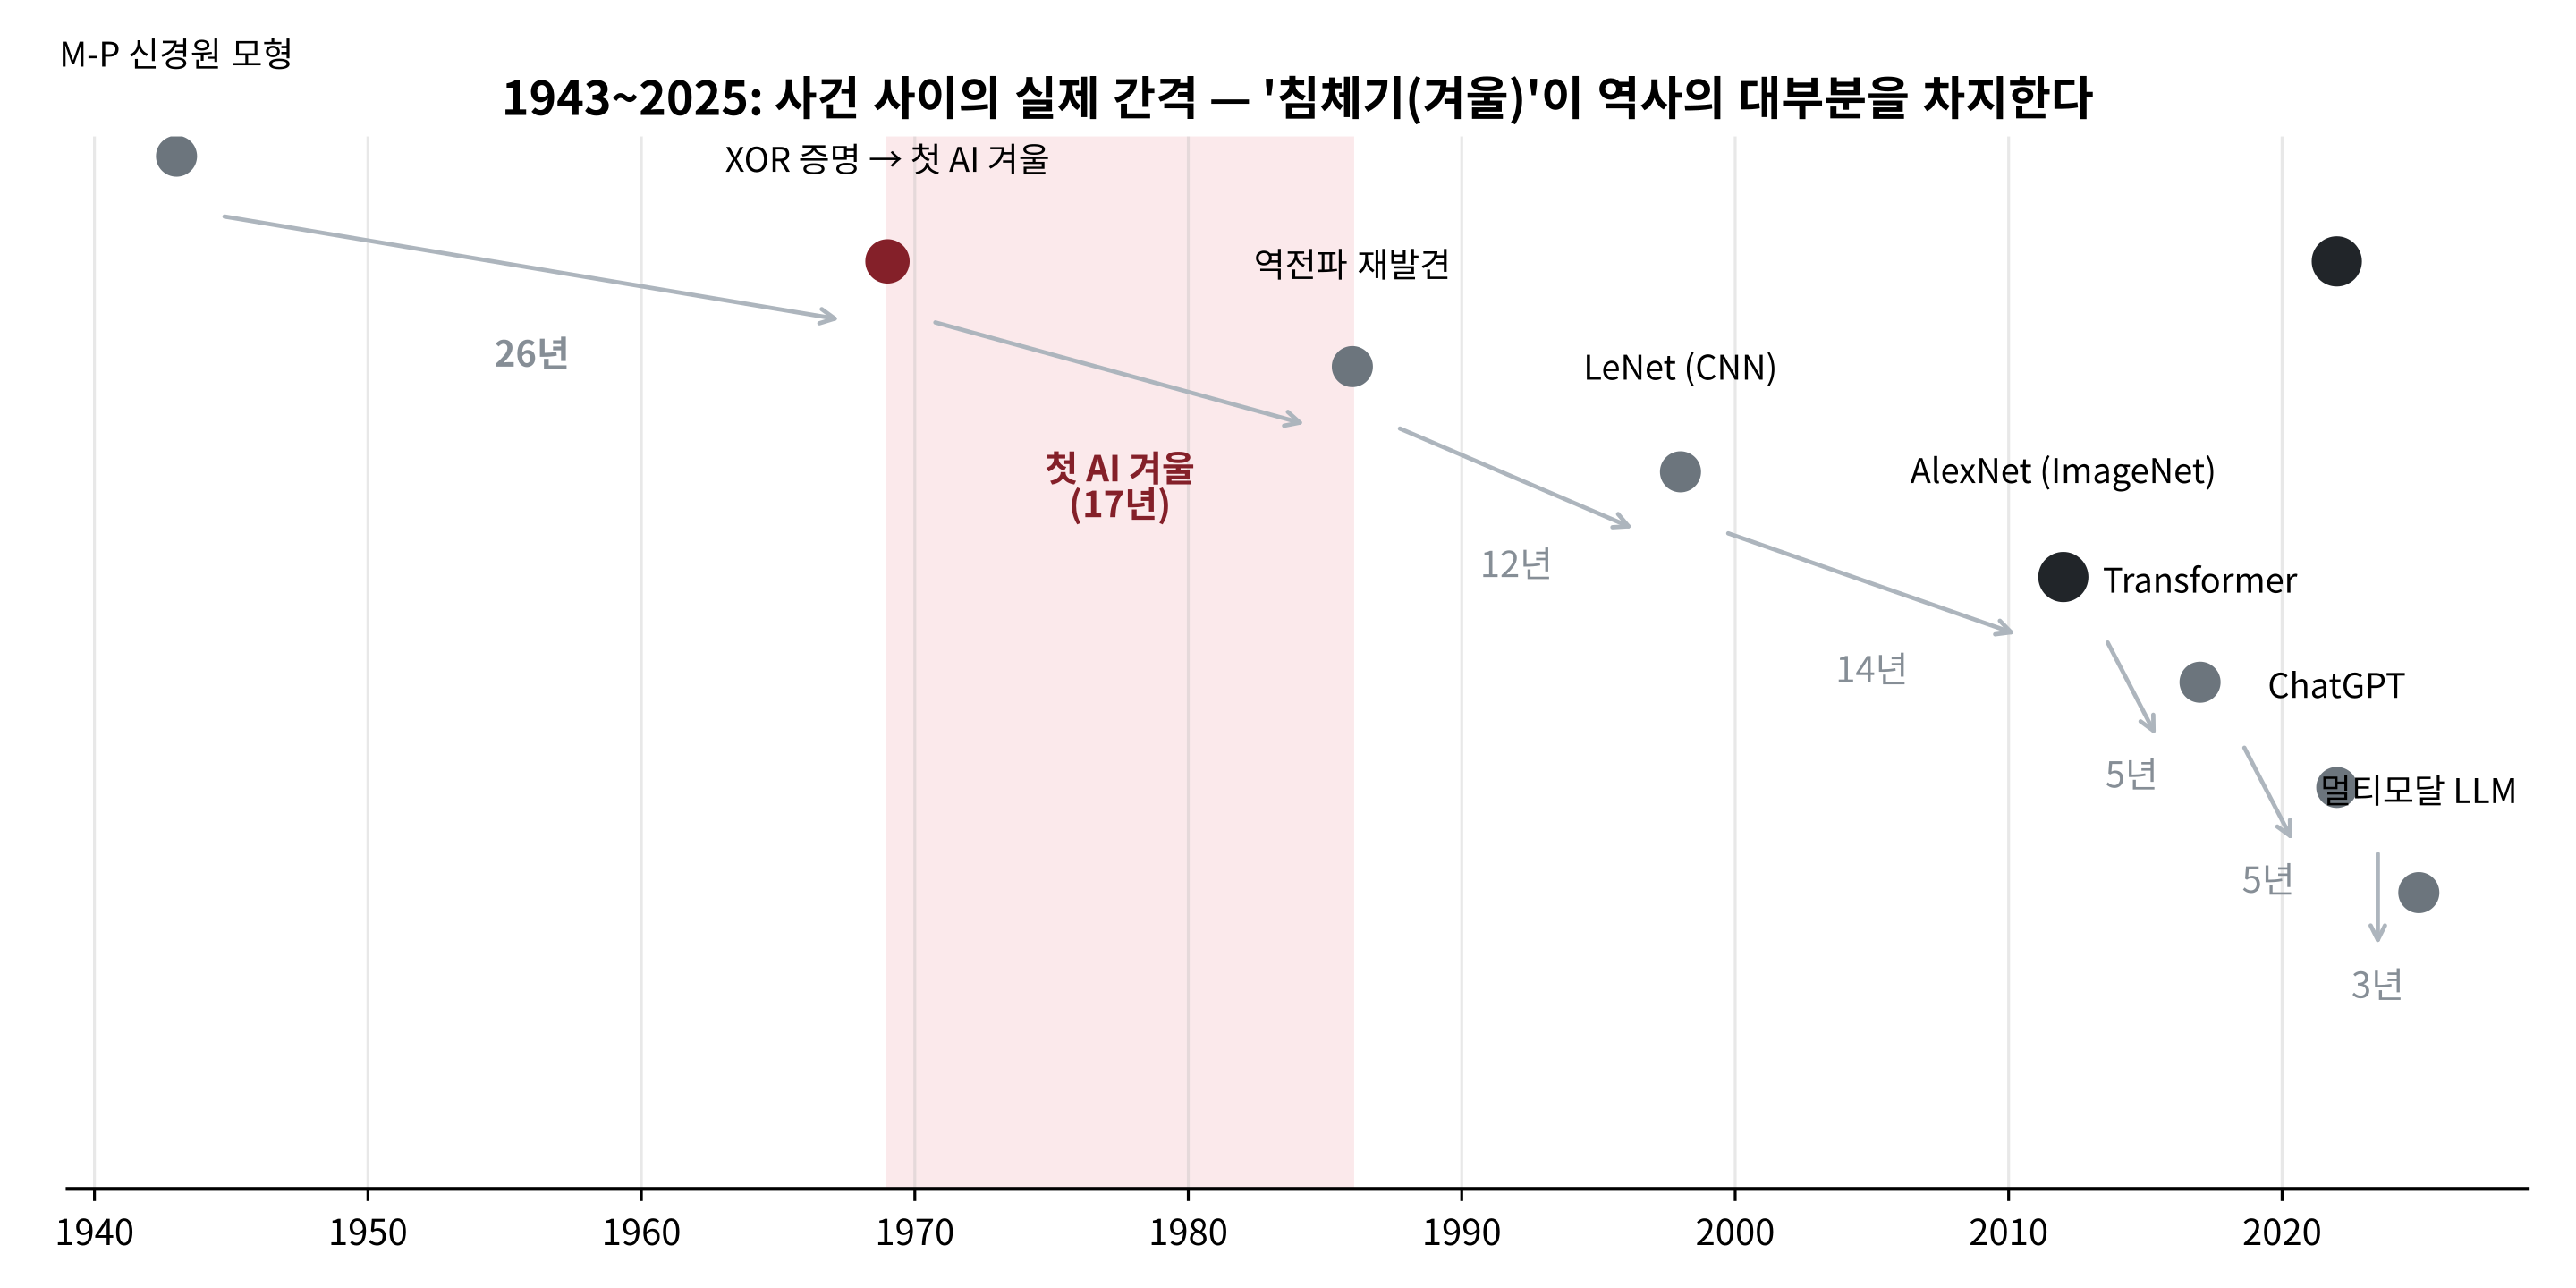
\includegraphics[width=\linewidth]{ch01_timeline_gaps.png}
      \vskip0.4em
      {\footnotesize 1969년 XOR 증명과 1986년 역전파 사이의 17년이
      가장 넓은 간격으로 보인다.}
    \end{column}
    \begin{column}{0.5\textwidth}
      \begin{itemize}
        \item 1943$\to$1969의 \textbf{26년}, 1969$\to$1986의 \textbf{17년} 같은
          긴 침체기가 역사의 상당 부분을 차지.
        \item \textbf{2012년 이후에만} 5년·5년·3년 간격이 반복된다.
        \item 표만 보면 안 와닿는 ``직선이 아니다''가 숫자로 보인다.
        \item 실습: 연표의 간격을 직접 계산하고, 2012년 이전 vs 이후의
          \textbf{평균 간격}을 비교.
      \end{itemize}
    \end{column}
  \end{columns}
\end{frame}

\begin{frame}{1969 --- 첫 겨울의 시작}
  \begin{itemize}
    \item 민스키·페퍼트가 단층 퍼셉트론은
      \textbf{XOR}(배타적 논리합, ``둘 중 정확히 하나만 참일 때만 참'')조차
      표현할 수 없음을 \textbf{수학적으로 증명}.
    \item ``아직 알고리즘이 부족하다''가 아니라, ``이 구조로는
      \textbf{원리적으로 불가능}하다''는 훨씬 강한 주장.
    \item 결과: 연구비가 끊기고 연구자 수가 급감 ---
      \kb{``첫 AI 겨울''}이 10년 넘게 이어짐.
  \end{itemize}
  \vskip0.6em
  \begin{block}{흥미로운 점}
    답(층을 여러 개 쌓으면 XOR도 표현 가능)은 \textbf{이미 알려진 수학} 안에
    있었지만, ``그 여러 층을 \textbf{어떻게 학습}시킬 것인가''라는
    \textbf{계산적 문제}가 안 풀려서 겨울이 그토록 길어졌다.
  \end{block}
\end{frame}

\begin{frame}{1986 --- 역전파가 겨울을 끝내다}
  \begin{itemize}
    \item 러멜하트·힌튼·윌리엄스(1986)가 역전파를 (재)발견.
    \item 여러 층을 가진 신경망도 \textbf{경사하강법으로 실제로
      학습}시킬 수 있다는 것이 드러나.
    \item 정확히 1969년의 한계(XOR)를 \textbf{실제로 풀어내는} 방법이었다.
  \end{itemize}
  \vskip0.6em
  \begin{block}{앞에서 다시 만난다}
    Ch.\,9에서 이 알고리즘을 손으로 유도해본다. 그 유도에 등장하는
    \textbf{연쇄법칙}은 1.3절에서 손으로 직접 계산해볼 바로 그 도구와
    \textbf{정확히 같은} 것이다.
  \end{block}
\end{frame}

\begin{frame}{2012 --- 딥러닝 시대의 개막}
  \begin{itemize}
    \item AlexNet은 1986년의 역전파, 1998년의 CNN(LeNet)과 근본적으로
      \textbf{다른 새 수학을 쓴 게 아니었다}.
    \item 결정적 차이: \textbf{GPU로 병렬 연산}하게 되면서 계산량이 감당
      가능해졌고, 인터넷 덕분에 ImageNet 같은 \textbf{대규모 라벨링된
      데이터셋}이 존재했다.
  \end{itemize}
  \vskip0.6em
  \begin{block}{교훈}
    ``좋은 아이디어가 있어도 \textbf{데이터와 계산 자원이 받쳐주지 않으면
    묻힐 수 있다}.''
  \end{block}
  \vskip0.4em
  \begin{itemize}
    \item 1969년의 증명 하나가 연구를 십수 년간 위축시켰다:
      \textbf{이론적 한계를 정확히 아는 것}이 때로는 ``무작정 더
      시도해보다'' 강력하다 --- 동시에 역전파는 바로 그 한계를 정확히
      풀어낸 해법이었다.
  \end{itemize}
\end{frame}

\begin{frame}{반복되는 패턴 --- 돌파구의 정체}
  \begin{block}{다수의 ``돌파구''는 새 수학이 아니다}
    이미 있던 아이디어(경사하강법, 연쇄법칙, 확률론)를
    \textbf{더 큰 데이터 · 더 많은 계산 자원} 위에서 \textbf{다시 조합}한
    것이다.
  \end{block}
  \vskip1em
  \begin{itemize}
    \item 1969 XOR 증명 $\to$ 17년 $\to$ 1986 역전파(바로 XOR의 해법).
    \item 1998 LeNet $\to$ 2012 AlexNet(같은 수학, GPU + ImageNet).
    \item \kb{이번 학기 목표}: 그 재사용되는 기본 아이디어 자체를
      \textbf{손으로 짚어보는 것}.
  \end{itemize}
\end{frame}

\begin{frame}{``왜 2012년이었을까'' --- 첫 번째 축: 계산}
  \begin{itemize}
    \item AlexNet은 2012년 최신 GPU 두 장(NVIDIA GTX 280)으로
      \textbf{약 5$\sim$11일} 걸리던 학습.
    \item 같은 모델을 당시 CPU 클러스터로 돌리면 \textbf{월 단위}로
      늘어나는 것이 일반적 추정.
    \item ``학습이 불가능했다''가 아니라 ``\textbf{학기가 끝나기 전에
      끝나지 않았다}'' --- 연구의 속도 경쟁에서는 사실상 같은 것.
  \end{itemize}
  \vskip0.6em
  \begin{block}{연상해야 할 도구: 무어의 법칙}
    집적회로의 성능이 대략 2년마다 배가. 고정된 ``한 학기 안에 끝나야
    하는'' 학습 시간 예산이 그대로라면, 1998년에는 LeNet 크기의 모델을
    돌리는 데 거의 다 썼겠지만, 2012년에는 같은 예산 안에
    \textbf{층과 폭이 훨씬 큰 모델}을 돌려볼 수 있었다.
  \end{block}
  \vskip0.4em
  신경망 연구에서 ``구조''와 ``계산''은 한 쪽만 커져서는 안 되는 한 쌍
  (Ch.\,9 역전파의 연산 비용을 손으로 셀 때 다시 등장).
\end{frame}

\begin{frame}{``왜 2012년이었을까'' --- 두 번째 축: 데이터}
  \begin{itemize}
    \item ImageNet: \textbf{약 140만 장}의 이미지에 \textbf{1000개 클래스}
      라벨을 붙인 데이터셋 (2009년 공개).
    \item 중요한 점: 라벨 대부분이 \textbf{일반인이 직접 매긴 것} ---
      인터넷과 크라우드소싱(아마존 메카니컬 터크) 플랫폼이 없었다면,
      100만 장 넘는 사진마다 ``고양이''·``셔터''를 붙이는 비용이
      \textbf{연구비를 압도}했을 것이다.
  \end{itemize}
  \vskip0.6em
  \begin{block}{``140만 장''과 ``2장 GPU''의 동시 출현}
    AlexNet의 승리는 두 축이 \textbf{동시에} 갖춰진 2012년에만 가능했던 것 ---
    어느 하나만 있었어도 그 해의 결과물은 달라졌다.
  \end{block}
  \vskip0.4em
  이번 학기 내내 등장하는 모든 모델이 이 ``두 축'' 위에 선다.
\end{frame}

\begin{frame}{세 번째 교훈: 라벨의 형태가 모델의 형태를 결정한다}
  \begin{itemize}
    \item 2012년의 패러다임 전환은 ``\textbf{사진 + 범주 라벨}''이라는
      \kb{지도학습}의 가장 전형적인 형태 위에서 일어났다.
    \item 정답이 없는 데이터만 있을 때(비지도학습, Ch.\,14$\sim$15),
      보상 신호만 있을 때(강화학습, ML2)에는 같은 GPU·데이터 축도
      중요하지만,
  \end{itemize}
  \vskip0.4em
  \kq{``어떤 신호로 학습하는가''에 따라 최적의 모델 가족 자체가 달라진다.}
  \vskip0.6em
  \begin{itemize}
    \item 1.2절에서 ``\textbf{데이터의 형태가 문제를 결정한다}''고 할 때
      뜻하는 바가 정확히 이것.
    \item 부수 효과: ``우리 데이터가 작으니 신경망은 아직 이르다'' 같은
      실무 판단이 왜 흔한지도 자연스럽게 이해된다.
  \end{itemize}
\end{frame}

\begin{frame}{이번 학기 로드맵 --- 8주 $\times$ 2 블록}
  \small
  \begin{columns}[T]
    \begin{column}{0.5\textwidth}
      \textbf{\color{ksablue}Block A (Ch.\,2--7): 고전 ML} --- 신경망 없이도
      강력; 지금도 정형(tabular) 데이터에서 자주 이긴다.
      \begin{tabular}{@{}cl@{}}
        \toprule
        2 & 회귀: 선형·로지스틱, 경사하강법, PR-AUC \\
        3 & 생성 관점 분류: 나이브베이즈와 GDA \\
        4 & 거리 기반·클러스터링: kNN, k-means, GMM/EM \\
        5 & SVM과 커널: 마진, 소프트 마진, 커널 트릭 \\
        6 & 정규화와 모델 선택: L1/L2, 교차검증 \\
        7 & 트리: 결정트리, 랜덤 포레스트, GBDT+SHAP \\
        8 & Block A 캡스톤 + 중간고사 대비 \\
        \bottomrule
      \end{tabular}
    \end{column}
    \begin{column}{0.5\textwidth}
      \textbf{\color{ksablue}Block B (Ch.\,9--16): 신경망 $\to$ 생성모델}
      \begin{tabular}{@{}cl@{}}
        \toprule
        9 & 신경망 기초: 퍼셉트론 한계, 역전파, 정규화 \\
        10 & CNN: 합성곱, 풀링, 탐지·분할·전이학습 \\
        11 & 시퀀스 모델: RNN, BPTT, LSTM/GRU \\
        12 & 어텐션과 트랜스포머: QKV, Multi-Head \\
        13 & 그래프 표현학습: Random Walk, Node2Vec, PageRank \\
        14 & 표현학습: PCA, word2vec, 임베딩 활용(RAG) \\
        15 & 잠재변수 생성모델: EM/GMM, VAE, GAN, Diffusion \\
        16 & Block B 캡스톤 + ML1 총정리 \\
        \bottomrule
      \end{tabular}
    \end{column}
  \end{columns}
  \vskip0.4em
  {\footnotesize 매 장 시작 전에 이 표를 펼쳐 ``지금 어디서 무엇을 배우고,
  어디로 이어지는지''를 확인하는 습관. (부록 Ch.\,17: LLM)}
\end{frame}

\begin{frame}{ML1과 ML2의 관계}
  \begin{itemize}
    \item \kb{강화학습과 로봇 시뮬레이션은 이번 학기(ML1)에서는 전혀
      다루지 않는다}.
    \item ML1과 ML2는 \textbf{서로 독립된 과목}으로 설계. ML2가 이 주제를
      처음부터 끝까지 전담.
    \item \textbf{ML1을 먼저 듣지 않아도 ML2를 바로 들을 수 있다} ---
      ML2 1주차에 필요한 신경망 기초를 압축해서 다시 짚어주기 때문.
  \end{itemize}
  \vskip0.6em
  \begin{block}{Block B의 내용 한 줄}
    역전파의 원리를 \textbf{손으로 유도}(Ch.\,9)한 뒤 CNN(Ch.\,10)까지
    기본기를 다지고, 시퀀스 모델$\to$Transformer$\to$LLM 계보(Ch.\,11$\sim$13)를
    훑은 뒤, 비지도학습(PCA·임베딩)과 VAE·GAN·Diffusion까지 생성모델로
    마무리(Ch.\,14$\sim$15).
  \end{block}
\end{frame}

\begin{frame}{이번 학기 쓸 도구들 (수학 + 코드)}
  \small
  \begin{tabular}{@{}lll@{}}
    \toprule
    도구 & 이 학기에서 쓰이는 곳 & 언제 처음 등장 \\
    \midrule
    numpy & 모든 실습의 기본. $w^\top x$, 행렬곱, 경사하강법 반복 & Ch.\,2 \\
    matplotlib & 손실 곡선, 결정경계, t-SNE/PCA 시각화 & Ch.\,2 \\
    pandas & EDA, 결측치 처리, 그룹별 통계 & Ch.\,6 (1.3절 예습) \\
    scikit-learn & 분류·회귀·클러스터링 모델의 표준 인터페이스 & Ch.\,2 \\
    PyTorch & 신경망·CNN·시퀀스 모델·VAE/GAN & Ch.\,9 \\
    Hugging Face & LLM 프롬프팅, 사전학습 모델 활용 & Ch.\,17 \\
    gymnasium & (ML2에서) 강화학습 환경 --- \textbf{ML1에서는 등장하지 않음} & --- \\
    \bottomrule
  \end{tabular}
  \vskip1em
  이 목록을 ``이번 학기에 \textbf{새로 배워야 할 것}''이 아니라,
  ``이 학기 내내 \textbf{반복해서 손이 갈 것}''으로 읽는다 ---
  완벽히 외우는 것보다, \textbf{필요할 때 10초 만에 꺼내 쓸 수 있는 것}이
  목표.
\end{frame}

\begin{frame}{실습 노트북의 역할}
  \begin{itemize}
    \item 각 절마다 붙는 실습 노트북(Colab 배지)은
      \textbf{``개념을 손으로 확인''}에 집중.
    \item 이번 절의 노트북: 연표의 \textbf{``격차''를 직접 계산},
      2012년 이전의 AI 겨울을 \textbf{시각화}, 도구 목록의 라이브러리가
      실제로 import 되는지 \textbf{확인}.
  \end{itemize}
  \vskip0.8em
  \begin{block}{미리 강조}
    ``어떤 모델을 쓰느냐''보다 \textbf{``도구가 손에 익었느냐''}가
    이 학기 전반부의 진짜 성패를 가른다.
  \end{block}
\end{frame}

\begin{frame}{자주 하는 실수: ``최신 모델''부터 잡기}
  \begin{itemize}
    \item 가장 흔한 실패 패턴: Transformer(Ch.\,12)·LLM(Ch.\,17)이
      ``산업에서 쓰는 것''이라는 이유로 \textbf{Block A를 건너뛰고
      Ch.\,12로 직행}.
    \item 실제 경험: 작은 네트워크의 손실이 안 떨어지는데
      (a) 데이터 스케일? (b) 학습률? (c) 구조 자체의 문제인지 구분 못
      하고 ``일단 층을 늘려보자''로 끝남.
    \item 한 달 뒤엔 \textbf{원인 모를 손실 곡선}만 남는다.
  \end{itemize}
  \vskip0.5em
  \begin{block}{디버깅이 불가능해지는 이유}
    Ch.\,6의 ``train/val/test 분리''와 Ch.\,2의 ``손실함수를 손으로
    한 번 계산'' 같은 \textbf{기초 도구가 없기} 때문이다.
  \end{block}
\end{frame}

\begin{frame}{실수의 본질 --- 그리고 로드맵이란}
  \begin{itemize}
    \item 본질: ``\textbf{최신 = 어렵다 = 배우면 실력이 된다}''는 착각.
    \item 실제로 최신 모델 논문의 한 줄 한 줄은 전부 Block A·B 기초
      (경사하강법, 시그모이드, 교차 엔트로피, 어텐션)의 \textbf{변형}.
    \item 기초가 없으면 논문을 ``읽는'' 게 아니라 ``\textbf{눈으로
      훑어보는}'' 것에 그침.
  \end{itemize}
  \vskip0.5em
  \begin{itemize}
    \item 반대로 Block A를 충실히 마치면 Transformer 논문을 읽을 때
      ``이 단락은 어텐션의 QKV를 다루는데, 12.1절의 QKV랑 같다''로
      \textbf{바로 위치를 잡을 수 있다}.
  \end{itemize}
  \vskip0.5em
  \kq{로드맵은 ``배울 것의 목록''이 아니라 ``어디서 어떤 기초가 다시
  쓰이는지''를 보여주는 지도.}
\end{frame}

\begin{frame}{실습: 나만의 학기 타임라인 만들기 (10분)}
  연표만 보는 것으로는 ``나''의 계획이 안 된다 --- 아래 3개를 노트로 직접
  짜기 (이 3개가 학기 내내 되돌아볼 ``나만의 로드맵''):
  \begin{enumerate}
    \item \textbf{연표 다시 쓰기}: 1943$\sim$2025 연표를 보지 않고
      ``이 사건이 왜 결정적이었는가''를 각 한 문장으로 다시 쓰기
      (막히면 1.2절 ``왜?'' 설명을 다시 보는 것이 정상).
    \item \textbf{교차점 찾기}: (a) 팀 프로젝트 발표가 있는 주간,
      (b) 새로 등장하는 수학 도구가 가장 많은 장, (c) 1.3절의 세 가지
      수학(내적·연쇄법칙·베이즈)이 \textbf{전부 한 번에} 등장하는 장을
      각각 하나씩 찾기.
    \item \textbf{도구 점검}: 지금 import 해볼 수 있는 것
      (numpy·matplotlib·pandas) vs 아직 설치/설명이 필요한 것
      (PyTorch, Hugging Face) 나눠보기.
  \end{enumerate}
  \vskip0.5em
  \begin{block}{힌트: (2)의 답}
    (b) = \kb{Chapter 9} --- 역전파는 \textbf{연쇄법칙을 수십 층에
    반복} 적용. \; (c) = \kb{Chapter 3} --- 나이브베이즈는
    \textbf{조건부 확률 + 베이즈 정리} + 가우시안 밀도의 \textbf{내적}
    형태.
    맞췄다면, 1.3절의 수학이 ``개별 장의 도구''가 아니라
    \textbf{``학기 전체를 관통하는 도구''}라는 감각이 잡힌 것.
  \end{block}
\end{frame}

\begin{frame}{확인 문제: 연표와 로드맵 (a)(b)}
  \textbf{이 절의 내용만으로} 답해볼 것 (답은 바로 아래).
  \begin{itemize}
    \item \textbf{(a)} ``2012년 AlexNet 승리의 원인은 앞서 나온 CNN(LeNet,
      1998)이 수학적으로 더 좋았기 때문.'' --- \kq{이 주장에 반대하려면
      어떤 근거 두 가지를 꺼내야 하는가?}
    \item \textbf{(b)} ``첫 AI 겨울이 10년 넘게 길었던 이유는, 답이
      이미 알려진 수학 안에 있었기 때문이다.'' ---
      \kq{인과가 잘못되었다면 어떻게 고쳐야 하는가?}
  \end{itemize}
  \vskip0.4em
  \begin{block}{답}
    (a) (1) AlexNet은 LeNet과 근본적으로 다른 새 수학을 쓰지 않았고,
    (2) 결정적 차이는 \textbf{GPU 병렬 연산 + 대규모 라벨링 데이터셋의
    동시 출현} --- ``수학의 우위''가 아니라 ``계산+데이터'' 축이 2012년에야
    갖춰진 것이 핵심 근거. \\[0.3em]
    (b) \textbf{인과가 반전}. ``답이 알려진 수학 안에 있었다''는 사실은
    겨울이 더 \textbf{길어}진 이유. 진짜 이유는 ``여러 층을 학습시킬
    계산적 문제(역전파)가 1986년 재발견까지 17년간 안 풀려 있었다''.
  \end{block}
\end{frame}

\begin{frame}{확인 문제 (c) + 자주 묻는 질문 1}
  \begin{itemize}
    \item \textbf{(c)} ``정형 데이터에서 지금도 신경망보다 자주
      이긴다''는 말은 어느 블록에 해당하는가? 한 문장으로 설명.
    \item \textbf{답}: \kb{Block A(Ch.\,2--7)} --- 회귀·나이브베이즈·kNN·
      SVM·정규화·트리 모델이 정형 데이터에서 아직까지도 신경망을 이기는
      경우가 흔하다는 것이 Block A를 학기 초반에 배치한 이유.
  \end{itemize}
  \vskip0.6em
  \textbf{Q. ML1과 ML2를 둘 다 들어야 하나요?}
  \begin{itemize}
    \item 아니다 --- 두 과목은 완전히 \textbf{독립} 설계.
    \item ML1: 데이터사이언스 $\to$ 고전 ML $\to$ 딥러닝 $\to$ 생성모델.
      ML2: 강화학습·로봇 시뮬레이션만 전담.
    \item \textbf{어느 쪽을 먼저 들어도, 혹은 하나만 들어도} 상관없다.
  \end{itemize}
\end{frame}

\begin{frame}{자주 묻는 질문 2: Block A를 건너뛰면?}
  \textbf{Q. Block A(고전 ML)를 안 배우고 Block B(신경망)로 바로
  넘어가면 안 되나요?}
  \begin{itemize}
    \item 이론적으로는 되지만, \textbf{권장하지 않는다}.
    \item Ch.\,6 정규화, Ch.\,7 트리 앙상블의 \textbf{``편향-분산
      트레이드오프''}와 ``train/val/test 분리''는 신경망에도
      \textbf{그대로 적용} --- Ch.\,9의 드롭아웃·배치정규화는 정확히
      같은 원리.
    \item 지금도 정형 데이터에서는 고전 ML이 신경망을 이기는 경우가
      흔해서 \textbf{실무에서 바로 쓸모}가 있다.
  \end{itemize}
  \vskip0.6em
  \textbf{Q. 수학이 약한데 따라갈 수 있나요?}
  \begin{itemize}
    \item 1.3절의 세 가지 수학(내적, 연쇄법칙, 베이즈 정리)이
      \textbf{사실상 전부}. 그 이상의 새 수학 도구는 거의 등장하지 않고,
    \item 대신 그 세 가지를 \textbf{점점 더 복잡한 상황에 반복 적용}하는
      것이 이번 학기의 실제 난이도. 낯선 표기가 나올 때마다 1.3절을
      참고하는 습관이면 충분.
  \end{itemize}
\end{frame}

\begin{frame}{자주 묻는 질문 3: 순서와 깊이}
  \textbf{Q. ML2를 먼저 듣고 ML1을 나중에 들어도 되나요?}
  \begin{itemize}
    \item \textbf{된다} --- 상호 선행 과목 관계가 아니라 완전 독립 설계.
      ML2는 1주차에 신경망 기초를 압축해서 다시 짚어줌.
    \item 다만 ML1의 ``정형 데이터에서 왜 아직도 고전 ML이 강한가''
      실무 감각은 ML2(로봇·강화학습 중심)에서는 다루지 않음 ---
      산업 현장에서 둘 다 쓸 예정이라면 \textbf{순서와 무관하게 두 과목
      다} 권함.
  \end{itemize}
  \vskip0.6em
  \textbf{Q. 모든 장을 같은 깊이로 배워야 하나요?}
  \begin{itemize}
    \item 아니다 --- 목표는 16개 장을 동일하게 깊게 이해하는 것이 아니라,
      매 장에서 \kq{``$h$는 무엇이고, $J$는 무엇이며, 어떻게
      최소화하는가''}라는 세 가지 질문에 답할 수 있는 정도.
    \item 특정 장(예: Ch.\,12)이 흥미로우면 더 깊게 파도 좋지만,
      그때도 Ch.\,9의 역전파가 먼저 잡혀 있어야 ``깊이 파는 것''과
      ``그저 보는 것''을 스스로 구분할 수 있다.
  \end{itemize}
\end{frame}

\begin{frame}{Python이 약한데? + 이번 차시 마무리}
  \textbf{Q. Python이 약한데 코드를 따라갈 수 있나요?}
  \begin{itemize}
    \item 기본 문법(변수, for 루프, 함수, 리스트)만 있으면 충분.
    \item 이 책은 의도적으로 개념 코드를 \textbf{순수 Python}(리스트 +
      for 루프)으로 짠 경우가 많음 --- ``벡터 연산 뒤에 숨은 for 루프를
      직접 눈으로 보기''가 우선.
    \item scikit-learn·PyTorch의 \emph{호출 이름}을 외우는 것이 목표가
      아니라, ``\textbf{이 함수가 안에서 뭘 하는가}''를 알고 쓰는 것이
      목표.
  \end{itemize}
  \vskip0.8em
  \begin{block}{1.1 마무리}
    어떤 모델을 쓸지보다 먼저 물어야 할 질문은 항상 같다:
    \kq{이 문제는 무엇을 데이터로 갖고 있고, 무엇을 맞히고 싶은가.}
  \end{block}
\end{frame}

% =================================================================
\section{1.2 머신러닝 문제 정식화와 세 갈래 분류}

\begin{frame}{문제를 푸는 게 아니라, 먼저 ``정의''부터}
  ``어떤 알고리즘을 쓸까''부터 고민하는 것이 흔한 착각 ---
  실전에서는 \textbf{순서가 반대}. 알고리즘보다 먼저 문제 자체를
  세 가지로 정의한다:
  \begin{enumerate}
    \item \kb{입력 $x$} --- 무엇을 \kb{특징(feature)}으로?
      (예: 집의 평수, 방 개수, 지어진 연도)
    \item \kb{출력 $y$} --- 무엇을 맞히나? \textbf{연속값(회귀)}인가
      \textbf{범주(분류)}인가?
    \item \kb{가설 $h$} --- 입력$\to$출력 함수를 어떤 \textbf{형태}로?
      (직선? 트리? 신경망?)
  \end{enumerate}
  \vskip0.4em
  \small
  \begin{columns}[T]
    \begin{column}{0.5\textwidth}
      \textbf{집값 예측}: $x$=평수·방·위치, \; $y$=거래가
      (\textbf{연속값}), \; $h$=\textbf{선형 함수}부터. 세 가지가 안
      정해지면 학습 목표 자체가 불분명.
    \end{column}
    \begin{column}{0.5\textwidth}
      \textbf{스팸 필터}: $x$=제목의 `무료'·발신자·느낌표 수
      (\textbf{특징의 벡터}), \; $y$=스팸(1)/정상(0)(\textbf{범주}).
      $x,y$ 의 \textbf{형태(연속 vs 범주)}가 다르니 \textbf{손실함수도
      달라야} 한다.
    \end{column}
  \end{columns}
  \vskip0.4em
  $x$ 를 잘못 고르면(예: 스팸 필터에 ``도착 요일''만 특징으로) 아무리
  좋은 알고리즘을 써도 $h$ 가 배울 \textbf{신호 자체가 없다}.
  \kq{``어떤 알고리즘이 가장 정확한가''보다 ``이 특징들이 애초에 정답과
  관련이 있는가''가 항상 먼저 물어야 할 질문.}
\end{frame}

\begin{frame}{학습(training)의 표기: $m$ 과 $(i)$}
  \begin{block}{학습의 정의}
    주어진 데이터 $(x^{(1)}, y^{(1)}), \dots, (x^{(m)}, y^{(m)})$ 에 대해
    $h(x^{(i)})$ 가 $y^{(i)}$ 에 최대한 가깝도록 $h$ 의
    \textbf{파라미터를 조정}하는 과정.
  \end{block}
  \vskip0.4em
  \begin{itemize}
    \item 위 첨자 $(i)$ = ``$i$ 번째 데이터 샘플'' (이 학기 내내 반복되는
      표기). $x^{(3)}$ = 세 번째 집의 특징 벡터.
    \item $m$ = 학습 데이터의 \textbf{전체 개수}(샘플 수).
    \item 예: 집 200채면 $m=200$, \; $x^{(37)}$ = 37번째 집의
      (평수, 방 개수, 연식), \; $y^{(37)}$ = 그 집의 실제 거래가.
  \end{itemize}
  \vskip0.4em
  학습은 ``학습 데이터를 \textbf{외우는 것}''이 아니라,
  \textbf{본 적 없는 201번째 집에도 일반화되는 규칙을 찾는 것} ---
  일반화 능력의 엄밀한 검증은 Ch.\,6.
\end{frame}

\begin{frame}{``정의를 먼저''의 역사: 세 시대}
  \small
  ``먼저 문제를 정의하라''가 추상적 교훈이 아니라 실제 역사에서 어떤
  결과를 만들었는지 세 시대로:
  \begin{itemize}
    \item \kb{1959 사무엘의 체커스 (Samuel, 1959)}: ``머신러닝''이라는
      말을 현대적 의미로 만든 논문. 기계를 ``플레이하게'' 하는 게
      아니라, ``\textbf{이 판국이 얼마나 좋은가}(평가함수, $y$)를
      \textbf{학습}하는 문제''로 \textbf{재정의} --- 판국 수가 사람이
      규칙을 전부 쓸 수 없을 만큼 많으므로 기계가 self-play에서 배우게.
      (이 재정의가 40년 뒤 \textbf{AlphaGo 계보}의 출발점.)
    \item \kb{1970s 전문가 시스템 (MYCIN, 1976) --- 역의 길}:
      의사들이 ``X 증상이면 Y를 의심하라''는 \textbf{규칙을 수백 개
      직접} 써넣은 감염 진단. 좁은 영역에서 전문의에 필적했으나,
      규칙 \textbf{유지보수가 사람에게}, 새 영역마다 수천 개를 다시
      사람이 --- 교훈: ``정의(=모든 규칙을 사람이 쓰는 것)가 사람에
      의존할수록, 상한도 사람의 역량에 갇히고 유지비도 비싸진다.''
    \item \kb{1998 LeNet과 우편 자동화 (Ch.\,10)}: ``입력: 손글씨
      숫자 이미지, 출력: 어느 숫자인가''. 사람이 형상(입력/출력)과
      특징을 설계하고, ``특징을 \textbf{어떻게 쓸 것인가}''는
      \textbf{기계가 데이터에서 학습} --- USPS 우편 분류에서
      ``사람은 문제만 정의하고 \textbf{기계가 세부 규칙을 배운다}''
      경로가 \textbf{확장성에 이긴 첫 대규모 증거}.
  \end{itemize}
  \vskip0.4em
  \begin{block}{세 시대가 주는 메시지}
    ``정의를 먼저 하라''는 \kq{매핑($x \to y$)의 \textbf{어느 부분을
    사람이 쓰고, 어느 부분을 기계가 배우게 할 것인가}를 정한다}는
    뜻. ``평가함수를 쓴다''$\to$ ``학습한다''(1959),
    ``인식 규칙을 쓴다''$\to$ ``특징을 학습한다''(1998) ---
    ``정의를 바꾸는'' 순간 불가능했던 문제가 가능해졌다.
  \end{block}
\end{frame}

\begin{frame}{실습: 세 문제를 스스로 정식화해보기}
  \small
  각 시나리오에 대해 $x$(입력 특징), $y$(출력), $h$ 의 대략적 형태(직선?
  규칙 기반? ``이번 학기에 배울 것'')를 노트에 적어보기.
  \begin{tabular}{@{}p{0.34\textwidth}p{0.6\textwidth}@{}}
    \toprule
    시나리오 & 힌트 (x / y / 갈래) \\
    \midrule
    \textbf{1. 신용카드 이상거래 탐지}\\ 매 결제가 사기인지를 즉시 판단 &
    $x$=결제 금액·시간·가맹점 종류, \; $y$=사기/정상(범주) $\to$ \textbf{분류} \\
    \textbf{2. 뉴스 기사 주제 자동 분류}\\ 정치/경제/스포츠/문화 태그 &
    $x$=기사 텍스트(나중에 단어 빈도·임베딩으로), \; $y$=4개 범주 중
    하나 $\to$ \textbf{분류(다중 클래스)} \\
    \textbf{3. 공장 설비 잔여수명 예측}\\ 진동·온도·가동시간 센서 &
    $x$=센서 측정값들, \; $y$=남은 일수(숫자) $\to$ \textbf{회귀} \\
    \bottomrule
  \end{tabular}
  \vskip0.6em
  세 문제 모두 ``\textbf{정답 라벨이 있고 $y$ 가 범주냐 숫자냐}''라는
  같은 질문 하나로 갈린다 --- 이번 학기 내내 새 문제를 만날 때마다
  가장 먼저 꺼내 쓸 도구.
\end{frame}

\begin{frame}{``정답''은 언제나 사람이 정한다: 라벨의 책임 I}
  $y^{(37)}$ 이 ``그 집의 \emph{실제} 거래가''라고 썼는데, ``실제''를
  오래 바라보자 ---
  \begin{itemize}
    \item $y^{(37)}$ 은 ``세상에서 정말 그 집의 가치''가 아니라,
      \kb{그 거래가 기록된 숫자}. 특수 사유(가족 간 거래, 급매)로
      비정상적으로 싸게 거래됐다면 ``가치''는 달라진다.
    \item 즉 라벨은 ``세상의 진실''이 아니라
      \textbf{``그 시점, 그 상황에서 사람이 기록한 값''}.
  \end{itemize}
  \vskip0.5em
  \begin{block}{실무 결과 1: 라벨의 정의는 팀 전체가 합의해야 한다}
    ``이탈 = 30일 이상 미접속''으로 정한 팀과 ``이탈 = 구독 해지''로
    정한 팀이 같은 데이터셋에 라벨을 매기면, \textbf{같은 고객에게 두
    라벨이 동시에} 붙을 수 있다. 정의가 일관성이 없으면 아무리 좋은
    $h$ 도 그 모순을 학습할 수 없다.
  \end{block}
\end{frame}

\begin{frame}{라벨의 책임 II --- 품질 확인과 세 갈래의 기준}
  \begin{block}{실무 결과 2: 라벨 품질은 EDA 단계에서 먼저 확인}
    라벨 분포가 \textbf{99:1}로 극단적으로 불균형하면 ``정확도 99\%''는
    사실상 \textbf{무의미}하다(전체를 ``비정상''으로 예측해도 99\%).
    해결은 라벨 재정의 · 재가중치 · 다른 평가지표(PR-AUC, Ch.\,2.3) ---
    출발점은 모두 ``\textbf{이 라벨이 정확히 무엇을 측정하는가}''를
    처음에 명확히 했는가.
  \end{block}
  \vskip0.6em
  \begin{itemize}
    \item 이 개념이 바로 다음 세 갈래 분류와 직결된다:
    \kq{라벨이 있는가 없는가가 \textbf{지도/비지도/강화}를 가르는
    기준}이기 때문이다.
  \end{itemize}
\end{frame}

\begin{frame}{세 갈래 분류: 무엇을 데이터로 갖고 있는가}
  머신러닝 문제는 세 갈래로 나뉜다 --- 알고리즘의 이름이 아니라,
  \textbf{어떤 형태의 데이터를 갖고 있고 어떤 신호로 학습하는가}로
  갈린다.
  \vskip0.5em
  \small
  \begin{tabular}{@{}llll@{}}
    \toprule
     & 데이터 형태 & 목표 & 이번 학기 예시 \\
    \midrule
    \kb{지도학습} & $(x, y)$ 쌍 & 새 $x$에 대한 $y$ 예측 & 회귀·분류, kNN,
      SVM, 트리, 신경망 \\
    \kb{비지도학습} & $x$ 만 & 데이터의 숨은 구조 발견 & k-means, PCA,
      EM/GMM \\
    \kb{강화학습} & 상태·행동·보상 & 누적 보상을 최대화하는 정책 &
      \textbf{ML1에서는 안 다룸} (ML2 전담) \\
    \bottomrule
  \end{tabular}
  \vskip0.6em
  {\footnotesize 강조: 기준은 ``얼마나 어려운 문제인가''가 아니라
  \textbf{``손에 쥔 데이터에 무엇이 적혀 있는가''}.}
\end{frame}

\begin{frame}{지도학습 내부: 판별적 vs 생성적}
  지도학습 안에서도 다시 두 갈래가 갈린다:
  \begin{columns}[T]
    \begin{column}{0.5\textwidth}
      \kb{판별적 (discriminative)}
      \begin{itemize}
        \item $P(y \mid x)$ --- ``$x$ 가 주어졌을 때 $y$ 의 확률''을
          \textbf{곧바로} 학습.
        \item 예: 회귀 · 로지스틱회귀 · SVM · 신경망.
      \end{itemize}
    \end{column}
    \begin{column}{0.5\textwidth}
      \kb{생성적 (generative)}
      \begin{itemize}
        \item $P(x \mid y)$ --- ``각 클래스가 데이터를 \textbf{어떻게
          만들어내는지}''를 먼저 학습.
        \item 그 다음 \textbf{베이즈 정리로 뒤집어} $P(y \mid x)$ 를
          얻는다. 예: Ch.\,3의 나이브베이즈·GDA.
      \end{itemize}
    \end{column}
  \end{columns}
  \vskip0.5em
  같은 문제를 \textbf{정반대 방향}에서 접근하는 두 철학의 차이는
  Chapter 3에서 자세히 다룬다.
\end{frame}

\begin{frame}{비지도학습과 강화학습}
  \begin{columns}[T]
    \begin{column}{0.5\textwidth}
      \kb{비지도학습} --- 정답 없이 \textbf{구조만} 주어짐
      \begin{itemize}
        \item ``이 고객들을 비슷한 성향끼리 묶어라''(\textbf{군집화}).
        \item ``1000개 특징을 정보 손실 최소로 10개로 줄여라''
          (\textbf{차원축소}).
        \item Chapter 14$\sim$15에서 다룸.
      \end{itemize}
    \end{column}
    \begin{column}{0.5\textwidth}
      \kb{강화학습} --- 정답이 아니라 \textbf{보상만} 주어짐
      \begin{itemize}
        \item 에이전트가 \textbf{시행착오}로 좋은 행동을 스스로 찾음.
        \item 체스·바둑: ``이 수가 정답이다''라고 알려주는 사람은
          없지만, ``이겼다/졌다''는 신호는 있다.
      \end{itemize}
    \end{column}
  \end{columns}
  \vskip0.5em
  \begin{block}{ML1에서는 다루지 않는다}
    ML1과 ML2는 서로 독립된 과목이고, ML2가 \textbf{강화학습과 로봇
    시뮬레이션을 처음부터 끝까지 전문으로} 다룬다.
    (ML2를 듣기 위해 ML1을 먼저 들을 필요는 없다.)
  \end{block}
\end{frame}

\begin{frame}{두 질문을 실제 시나리오에}
  \small
  \begin{tabular}{@{}p{0.36\textwidth}cll@{}}
    \toprule
    시나리오 & Q1: $y$ 가? & Q2: 보상이? & 갈래 \\
    \midrule
    지난 분기 매출로 다음 분기 매출 예측 & 있음(매출 숫자) & --- &
      지도·\textbf{회귀} \\
    고객 구매 기록만으로 ``비슷한 취향'' 그룹 발견 & 없음 & 없음 &
      \textbf{비지도} \\
    드론이 충돌 없이 목표지에 도착하도록 경로 학습 & 없음 & 있음(도착/
      충돌 신호) & \textbf{강화} \\
    X-ray 사진으로 폐렴 유무 판별 & 있음(의사 진단) & --- &
      지도·\textbf{분류} \\
    \bottomrule
  \end{tabular}
  \vskip0.8em
  \begin{block}{왜 두 단계인가}
    $y$ 가 있으면 강화학습의 구조(상태·행동·보상)가 존재할 여지가
    \textbf{아예 없다} $\Rightarrow$ 질문 1이 먼저.
    2를 먼저 던지면 $y$ 가 있는 데이터에서 보상을 \textbf{억지로}
    만들 위험 --- ``매출이 올랐으니 보상 +1''의 순간,
    \textbf{보상 설계(reward shaping)}의 가장 흔한 함정(행동$\to$결과
    인과가 모호).
  \end{block}
\end{frame}

\begin{frame}{세 갈래를 대표하는 유명한 시스템}
  \begin{itemize}
    \item \kb{지도 --- ImageNet/AlexNet}: 100만 장이 넘는 사진 각각에
      사람이 미리 ``고양이''·``자동차'' 같은 \textbf{정답 라벨}을
      붙여뒀다. 라벨이 없었으면 이 방식 자체가 \textbf{불가능}.
    \item \kb{비지도 --- 넷플릭스/스포티파이 군집화}: ``당신과 비슷한
      취향의 사람이 좋아한 콘텐츠''를 추천할 때, ``이 사람은 그룹 3에
      속한다''는 \textbf{정답 라벨은 어디에도 없다}. 시청·청취 기록만으로
      비슷한 패턴을 알고리즘이 스스로 묶어냄.
    \item \kb{강화 --- AlphaGo}: 바둑의 ``정답 수''를 사람이 알려준 적
      없다(최선의 수를 사람도 모른다). 대신 ``\textbf{이겼다(+1)/
      졌다(-1)}''라는 보상만으로 스스로 수백만 판을 두며 정책 개선
      --- ML2에서 처음부터 다룸.
  \end{itemize}
\end{frame}

\begin{frame}{같은 데이터, 다른 갈래: ``라벨 관점''이 문제를 바꾼다}
  \small
  한 이커머스: 각 고객의 (연령, 지역, 월 구매 횟수, 평균 구매액,
  최근 90일 방문 빈도) + ``지난 30일 구독 해지 여부(1/0)'' 라벨.
  \begin{enumerate}
    \item \textbf{그냥 있는 그대로} --- $y$ = 해지 여부 예측 $\to$
      \kb{지도학습·분류}(이탈 예측 모델, Ch.\,2$\sim$7의 도구 중 하나).
    \item \textbf{라벨만 버리면} --- 특징만으로 ``비슷한 구매 성향을
      묶어라'' $\to$ \kb{비지도학습·군집화}. 군집이 나중에 ``이 군집의
      이탈 확률이 높다''는 통찰로 이어질 수도 --- \textbf{라벨을 버린
      비지도가 라벨을 쓴 지도보다 넓은 시야}를 줄 수 있음.
    \item \textbf{한 걸음 더} --- 매 주 쿠폰(10\%/20\%/무료배송)을
      직접 결정하고, 다음 주 매출(보상)을 관찰하며 \textbf{시행착오}로
      개선 $\to$ \kb{강화학습}. ``이 고객에게 이 쿠폰이 정답''이라는
      라벨은 어디에도 없고, \textbf{보상(매출 변화)만}.
  \end{enumerate}
  \vskip0.4em
  \kq{같은 원본 데이터셋에서, 무엇을 라벨로 볼 것인가에 따라 \textbf{세
  갈래 모두가} 만들어진다.}
  \vskip0.3em
  {\footnotesize ML1의 챕터가 지도(Ch.\,2$\sim$13) + 비지도
  (Ch.\,14$\sim$15) 두 갈래에 머무는 이유: 강화학습은 ``정답이 아예
  없고 보상만 있다'' --- 데이터의 형태 자체가 \textbf{근본적으로
  달라} 별도 과목(ML2)을 통째로 할애할 만큼 다르다.}
\end{frame}

\begin{frame}{회귀 vs 분류: 같은 모델, 다른 출력}
  지도학습은 다시 출력이 \textbf{연속값이냐 범주냐}로 나뉜다:
  \begin{itemize}
    \item \kb{회귀(regression)}: \textbf{숫자}를 예측 (집값, 기온).
    \item \kb{분류(classification)}: \textbf{범주}를 예측 (스팸/정상,
      개/고양이/새).
  \end{itemize}
  \vskip0.4em
  같은 선형 모델 $w^\top x + b$ 라도, \textbf{출력을 그대로 쓰면 회귀},
  \textbf{시그모이드를 씌워 0$\sim$1 확률로 해석하면 분류} (둘 다
  Ch.\,2). 앞으로 몇 장 동안 반복되는 패턴:
  \begin{block}{모델 구조는 비슷한데, 출력을 해석하는 방식과
  손실함수(loss function)만 문제에 맞게 바뀐다.}
  \end{block}
  \vskip0.4em
  \begin{itemize}
    \item 예: 학습된 $w = [0.5, -2.0]$, \; $b = 1.0$, \; 새 데이터
      $x = [3, 0.5]$.
      \[w^\top x + b = 0.5 \times 3 + (-2.0) \times 0.5 + 1.0
        = 1.5 - 1.0 + 1.0 = 1.5\]
  \end{itemize}
\end{frame}

\begin{frame}{같은 $1.5$, 두 가지 읽기 --- 시그모이드}
  \begin{itemize}
    \item \kb{회귀로} 쓰면: 결과 $1.5$ 를 \textbf{그대로 예측값}으로
      읽음 (예: ``이 집은 1.5억 원'').
    \item \kb{분류로} 쓰면: 정확히 같은 $1.5$ 를 시그모이드
      $\sigma(z) = 1/(1+e^{-z})$ 에 통과시켜 $\sigma(1.5) \approx 0.82$
      $\to$ ``이 이메일이 \textbf{스팸일 확률 82\%}''로 읽음.
  \end{itemize}
  \vskip0.5em
  \kq{가중치 $w$, 편향 $b$, 입력 $x$ 는 완전히 동일한데, 오직
  ``출력을 어떻게 해석할 것인가''만 바뀌었다.}
  \vskip0.6em
  \begin{block}{시그모이드가 왜 필요한가}
    $z$ 는 $(-\infty, +\infty)$ 의 아무 값이나 나온다. ``확률''로
    읽으려면 0과 1 사이가 필요하고, $z$ 가 커질수록 1에, 작을수록 0에
    \textbf{부드럽게(미분 가능하게)} 가까워져야 한다 --- 그래야
    Ch.\,2 경사하강법에서 미분이 잘 되기 때문. 시그모이드는 이 두
    성질을 동시에 만족하는 \textbf{가장 간단한} 함수.
  \end{block}
\end{frame}

\begin{frame}[fragile]{링크 함수 + 실습: 같은 계산, 두 가지 해석}
  ``출력 해석을 확률로 바꾸는'' 단계 = \kb{링크 함수}: 회귀 =
  \kb{항등 함수}($z$ 를 그대로), 이진 분류 = \kb{시그모이드}.
  Ch.\,2에서 이 차이로 \textbf{손실함수가 어떻게 달라지는지}
  직접 유도(MSE vs 교차 엔트로피).
  \begin{lstlisting}
import math

def sigmoid(z):
    return 1 / (1 + math.exp(-z))

w = [0.5, -2.0]
b = 1.0
x = [3, 0.5]

z = sum(wi * xi for wi, xi in zip(w, x)) + b
print("z =", z)                        # 1.5
print("회귀로 읽으면:", z)               # 1.5 (그대로 예측값)
print("분류로 읽으면:", sigmoid(z))      # 약 0.818 (양성 클래스일 확률)
\end{lstlisting}
  \vskip0.2em
  {\footnotesize $z$ 를 만드는 코드는 \textbf{한 줄로 똑같고},
  \texttt{sigmoid()} 를 씌우느냐 마느냐 \textbf{한 줄 차이}가
  회귀/분류. Ch.\,2: 이 $z$ 를 만드는 $w, b$ 자체를 \textbf{데이터로
  학습}(경사하강법). Colab: 2D 점군을 회귀선 vs 분류 경계로 나란히,
  \texttt{classify\_dataset()} 작성.}
\end{frame}

\begin{frame}{공통 뼈대: 손실함수 $J$ 를 정의하고 최소화한다}
  지금부터 배우는 거의 모든 알고리즘은 다음 \textbf{두 단계 틀}을 따른다:
  \begin{enumerate}
    \item 모델이 얼마나 틀렸는지를 \textbf{숫자 하나로 요약}하는
      \kb{손실함수} $J(w)$ 를 정의.
    \item $J(w)$ 를 \textbf{최소화}하는 $w$ 를 찾는다 (대개
      \textbf{경사하강법}, Ch.\,2).
  \end{enumerate}
  \vskip0.5em
  \begin{itemize}
    \item 회귀의 손실(평균제곱오차)과 분류의 손실(교차 엔트로피)은
      \textbf{형태가 다르지만}, ``틀린 정도를 수치화하고 그걸
      줄인다''는 \textbf{구조 자체는 동일}.
    \item Ch.\,2 선형·로지스틱회귀, Ch.\,5 SVM(힌지 손실), Ch.\,9 신경망
      (역전파로 손실 최소화)까지 --- $h$ 의 형태와 $J$ 의 모양은
      알고리즘마다 다르고, \textbf{절차 자체는 똑같이 반복}.
  \end{itemize}
  \vskip0.4em
  \kq{매 챕터에 습관적으로 던질 세 질문: ``$h$ 는 무엇이고, $J$ 는
  무엇이며, 어떻게 최소화하는가.''}
\end{frame}

\begin{frame}{세 갈래를 가르는 ``데이터의 형상'' --- 표로 보면 된다}
  \begin{itemize}
    \item \kb{지도}: \textbf{2개 블록} --- 왼쪽 $x$ 블록(특징 열),
      오른쪽 $y$ 블록(라벨 1열). 행 $m$ 개, 열 $(p+1)$ 개. 핵심 질문:
      ``라벨 열이 있는가?''
    \item \kb{비지도}: \textbf{1개 블록} --- $x$ 블록만 있고 라벨
      \textbf{열이 없다}. 행 $m$ 개, 열 $p$ 개. 목표: ``구조를 찾자''.
    \item \kb{강화}: 형상 자체가 다름 --- 각 행이
      $(s_t, a_t, r_t, s_{t+1})$ 4개 필드(상태, 행동, \textbf{보상},
      다음 상태)를 가진 \textbf{경험 튜플} 목록. 라벨 열 대신
      \textbf{보상 열}이 있다.
  \end{itemize}
  \vskip0.5em
  \begin{block}{``라벨 열''과 ``보상 열''의 차이}
    라벨 = ``이 입력 $x$ 에 대한 \textbf{정답}''. \; 보상 = ``이
    행동을 취한 \textbf{결과}가 좋았는가''를 숫자로 알려줄 뿐,
    ``정답 행동은 무엇이었는가''를 \textbf{아주 느리고 부분적으로}만
    알려준다. 이것이 세 갈래의 가장 근본적인 차이 (ML2에서 본격 다룸).
  \end{block}
\end{frame}

\begin{frame}{자주 하는 실수: 정의를 건너뛰고 알고리즘부터}
  \begin{itemize}
    \item 사례: 스타트업이 ``이탈 예측 모델 만들자''는 목표만 갖고
      ``\textbf{그럼 신경망을 쓸까, XGBoost를 쓸까?}''부터 논의.
    \item 몇 주 뒤 모델은 완성됐지만 \textbf{성능이 엉망} ---
      ``이탈''의 정의(30일 미접속? 구독 해지? 환불 요청?)조차
      \textbf{팀마다 다르게} 이해하고, $y$(라벨) 자체가 일관성 없이
      매겨져 있었음.
  \end{itemize}
  \vskip0.5em
  \kq{알고리즘 선택에 쓴 시간보다, $y$ 를 정의하는 데 쓴 시간이 훨씬
  적었던 것이 진짜 원인.}
  \vskip0.5em
  \begin{itemize}
    \item ``어떤 모델이 가장 정확할까''는 \textbf{프로젝트 중반 이후}의
      질문. 초반에 가장 먼저 답해야 할 질문은 ``$x$ 는 무엇이고, $y$ 는
      정확히 무엇이며, 그 정의에 \textbf{모두가 동의하는가}''.
    \item Ch.\,8, 16 팀 프로젝트: 데이터를 내려받자마자 모델링에
      뛰어들지 말고, 이 세 가지 질문에 \textbf{팀 전체가 명시적으로}
      답을 적어두기.
  \end{itemize}
\end{frame}

\begin{frame}{실수 두 번째: ``라벨 없으니 비지도겠지''}
  ``라벨이 없다''는 \textbf{현상}이 ``비지도학습이 맞는 문제''라는
  \textbf{결론}으로 바로 이어지지는 않는다.
  \begin{itemize}
    \item \textbf{``라벨이 비싸서 못 만들었다'' vs ``라벨이
      원리적으로 없다''}: X-ray 폐렴 판별에서 ``폐렴/정상'' 라벨은
      의사가 매겨야 해 비싸고 느리다. 비지도로 푸는 것은 ``라벨을
      만들지 않겠다''는 \emph{선택}이지 ``원리적으로 없다''가 아님
      $\to$ 대개는 ``\textbf{라벨을 일부라도} 만들 수 있는가''를 먼저
      고민 (의사 10장만 라벨 + 나머지 비지도 = \textbf{반지도학습},
      Ch.\,9$\sim$10에서 간접 다룸).
    \item \textbf{``보상이 있긴 한데 '라벨'인 줄 알았다''}:
      ``재구매 여부''는 \textbf{라벨}(지도)로 쓸 수도, ``또 샀으니
      +1''이라는 \textbf{보상}(강화)으로 읽을 수도 --- Q1/Q2로 다시
      확인.
  \end{itemize}
\end{frame}

\begin{frame}{확인 문제: 이 시나리오는 어떤 갈래인가 (a)$\sim$(d)}
  \small
  각 사례를 읽는 지도/비지도/강화, 그리고 회귀/분류까지 판단:
  \begin{tabular}{@{}p{0.52\textwidth}p{0.42\textwidth}@{}}
    \toprule
    시나리오 & 답 \\
    \midrule
    (a) 넷플릭스가 시청 기록(장르, 시청 시간)만으로 ``비슷한 취향 그룹''
    자동 탐색 & \textbf{비지도} --- ``그룹 3에 속한다''는 정답 없이
      구조(비슷한 패턴)만으로 탐색 \\
    (b) 은행이 과거 대출자(소득, 신용점수, 상환 여부)로 ``새 신청자가
    상환할지'' 예측 & \textbf{지도·분류} --- ``상환함/못함'' 범주 정답이
      이미 붙어 있음 \\
    (c) 로봇 청소기가 배터리 아끼며 방을 최대한 깨끗이 청소하도록
    스스로 수백 번 시행착오 & \textbf{강화} --- ``이 방향이 정답''을
      알려주는 사람 없이 ``청소 면적''·``남은 배터리'' 보상으로 정책
      개선 (ML2에서 본격) \\
    (d) 부동산 플랫폼이 매물 정보로 예상 거래가를 \textbf{숫자}로
    예측 & \textbf{지도·회귀} --- $y$(거래가)가 범주가 아니라 연속
      숫자 \\
    \bottomrule
  \end{tabular}
  \vskip0.4em
  {\footnotesize 기준이 항상 같다: ``정답 라벨이 있는가'', 있다면
  ``숫자인가 범주인가'' --- 질문 두 개로 어떤 문제든 분류할 수 있다.}
\end{frame}

\begin{frame}{확인 문제 (e)(f)(g) + 1.2 마무리}
  \small
  \begin{itemize}
    \item \textbf{(e)} 게임사가 ``플레이어가 다음 주에도 접속할
      것인가''를 과거 행동 로그로 예측 $\to$ \kb{지도·분류}
      (``다음 주에도 접속'' \textbf{라벨}이 이미 붙어 있음).
    \item \textbf{(f)} 같은 게임사가 ``지금 어떤 아이템을 쓰면 장기
      승률에 좋은지''를 실제 플레이(시행착오)로 학습 $\to$
      \kb{강화} (``지금의 정답 행동'' 라벨은 없고 ``승리/패배''
      \textbf{보상}만). (e)(f)는 \textbf{같은 게임 로그}를 갖고,
      예측 대상을 보는 관점에 따라 갈래가 바뀜.
    \item \textbf{(g)} SNS가 친구 관계 \textbf{그래프만} 갖고
      ``비슷한 커뮤니티''를 자동 탐색 $\to$ \kb{비지도}
      (``커뮤니티 5에 속한다''는 라벨 없이 연결 밀도 구조로 탐색).
  \end{itemize}
  \vskip0.4em
  \textbf{Q. ``지도 vs 비지도''와 ``회귀 vs 분류''는 같은 기준인가?}
  아니다 --- \textbf{수직} 관계. 지도가 ``라벨이 있는가?''로 먼저
  갈리고, 그 안에서 ``숫자인가 범주인가?''로 갈린다. 비지도/강화는
  회귀/분류 구분 \textbf{그 자체가 없다}.
  \vskip0.4em
  {\footnotesize 반지도(라벨 1\% 수준)·자기지도(라벨이 데이터에서
  자동 생성)는 세 갈래의 \textbf{경계} 변종 (Ch.\,9$\sim$10, 14$\sim$15에서
  간접 등장). ``보상''이 있어도 무조건 강화가 아님 ---
  \textbf{보상의 인과성}(행동$\to$결과)이 성립할 때만 신호 (ML2
  reward shaping).}
\end{frame}

\begin{frame}{1.2 마무리}
  \begin{block}{핵심 질문}
    어떤 문제를 만나든, 첫 질문은 항상 같다:
    \kq{손에 쥔 데이터에 무엇이 적혀 있는가 --- 그리고 그것을
    ``라벨''으로 볼 것인가, ``보상''으로 볼 것인가, 아니면
    ``구조''로만 볼 것인가.}
  \end{block}
  \vskip0.6em
  \begin{itemize}
    \item $x, y, h$ 로 \textbf{먼저 정의}하고, 두 질문으로 세 갈래를
      가르고, 지도 안에서는 ``연속/범주''로 회귀/분류를 가른다.
    \item 회귀 vs 분류 = \textbf{같은 모델, 다른 출력}
      (항등 링크 vs 시그모이드).
    \item 모든 알고리즘의 뼈대 = \textbf{$J$ 를 정의하고 최소화}
      ($h$, $J$, 최소화 방법의 세 질문).
  \end{itemize}
\end{frame}

% =================================================================
\section{1.3 데이터사이언스 파이프라인과 사전지식 리뷰}

\begin{frame}{모델은 파이프라인의 한 조각일 뿐}
  1.2절은 ``모델을 어떻게 정의하는가''였지만, 실전에서 모델 학습은
  전체 작업의 \textbf{작은 일부}에 불과하다. 실제 데이터 프로젝트의
  순환:
  \begin{enumerate}
    \item \kb{수집} --- 어디서 데이터를 구할 것인가. Ch.\,8, 16 팀
      프로젝트에서는 Kaggle, UCI ML Repository, Hugging Face Datasets 등
      공개 저장소를 주로 사용. 실무에선 ``이 데이터를 이 목적으로 써도
      되는가''(라이선스, 개인정보) 확인도 포함 --- 캐글 대회 데이터라도
      \textbf{상업적 재사용이 금지}된 경우가 흔함.
    \item \kb{정제} --- \textbf{결측치} · \textbf{중복} ·
      \textbf{이상치}를 처리 (현실 데이터는 거의 항상 지저분).
    \item \kb{탐색적 데이터 분석(EDA)} --- 모델을 만들기 전에
      분포·상관관계·클래스 비율을 \textbf{눈으로} 확인. 이 단계의 발견이
      어떤 모델을 고를지까지 결정 (예: 99:1 불균형 $\to$
      정확도 대신 PR-AUC, Ch.\,2.3).
    \item \kb{모델링} --- 1.2절에서 정식화한 문제에 맞는 $h$ 를 고르고
      학습. 이번 학기 대부분의 장.
    \item \kb{평가} --- \textbf{학습에 쓰지 않은} 데이터로 성능 검증
      (엄밀한 원리는 Ch.\,6). 나쁘면 4단계(다른 모델?)로만 돌아가지
      않고 \textbf{1$\sim$3단계로 되돌아가야} 할 수도 ---
      ``모델이 나쁜 것''이 아니라 ``데이터가 애초에 그 신호를 담고 있지
      않은 것''일 수 있기 때문.
  \end{enumerate}
\end{frame}

\begin{frame}{왜 이 순서인가 --- 결함은 아래로 ``증폭''된다}
  \begin{itemize}
    \item \kb{모델링은 다섯 단계 중 하나일 뿐} --- 처음 배우는 이들이
      가장 자주 간과하는 점. 캐글 프로젝트에서 결측치 처리 + EDA에
      드는 시간이 모델 코드보다 \textbf{긴 경우가 흔함}.
    \item 파이프라인 앞 단계의 결함은 뒤에서 아무리 좋은 모델을 써도
      \textbf{수리되지 않는다}.
  \end{itemize}
  \vskip0.5em
  \begin{itemize}
    \item \textbf{결측치 미처리}: 모델이 ``결측 처리의 흔적''을
      \textbf{정답인 양} 학습.
    \item \textbf{중복 행}: 같은 사례를 여러 번 외워 ``중요도가
      부풀려진'' 데이터.
    \item \textbf{미래 정보}(예: ``거래 완료 여부''를 특징으로 쓰는
      집값 예측): 훈련 때는 비현실적으로 정확하고 \textbf{실전에만
      무너지는}, 디버깅이 거의 불가능한 모델.
  \end{itemize}
  \vskip0.4em
  \begin{block}{실무 경험자들의 일치된 증언}
    파이프라인은 위에서 아래로 흐르되,
    \kq{결함은 위에서 아래로 \textbf{``증폭''}}되는 구조.
  \end{block}
\end{frame}

\begin{frame}{자주 하는 실수: EDA를 건너뛰고 바로 모델링}
  1.2절의 ``정의 없이 알고리즘부터 고르지 말라''가 이 파이프라인에도
  그대로 적용된다.
  \begin{itemize}
    \item 흔한 실패 패턴: 데이터를 내려받자마자 \texttt{df.head()} 만
      한 번 찍어보고 바로 \texttt{model.fit(X, y)} 를 돌림.
    \item 나중에 성능이 이상해서 다시 들여다보면:
    \begin{itemize}
      \item 가격 열에 \textbf{음수값}이 섞여 있었거나,
      \item 한 지역이 전체의 \textbf{90\%}를 차지해 다른 지역은
        사실상 학습이 안 됐거나,
      \item 특정 열이 \textbf{``미래 정보''}(예측 시점엔 알 수 없는 값)
       를 담고 있어 학습 때만 비현실적으로 정확했던 것.
    \end{itemize}
  \end{itemize}
  \vskip0.5em
  \begin{block}{EDA 10분의 가치}
    전부 \texttt{df.describe()}, \texttt{df.corr()}, 그룹별 통계 몇 줄
   만 먼저 찍어봤어도 모델을 돌리기 \textbf{전에} 잡을 수 있었던 것.
    EDA에 쓰는 10분이, 잘못된 가정 위에 쌓은 모델을 디버깅하는
    \textbf{몇 시간}을 아껴준다.
  \end{block}
\end{frame}

\begin{frame}{유명한 사고: Aha! 데이터셋 (Wolpert \& Kibler, 1992)}
  머신러닝 역사에서 \textbf{데이터 품질}의 중요성을 보여주는 가장
  유명한 사례:
  \begin{itemize}
    \item 1992년, SRI 국제 AI 센터의 \textbf{Wolpert와 Kibler} ---
      ``\emph{Do We Know the Data We're Using?}'' (Wolpert \& Kibler,
      1992).
    \item 당시 표준 벤치마크 UCI의 ``Aha!'' 데이터셋을 들여다봤더니,
      \textbf{동일한 특징 벡터의 행이 서로 다른 정답 라벨로 2개 이상}
      들어 있는 경우가 \textbf{100건}.
    \item 같은 입력에 서로 모순되는 정답이 두 개면, 아무리 완전한
      모델이라도 그 쌍 중 \textbf{적어도 한 건은 틀릴 수밖에} 없다
      (수학적 문제).
  \end{itemize}
  \vskip0.4em
  \begin{block}{교훈}
    ``어떤 알고리즘이 더 좋은가'' 비교 논문들에, 알고리즘이 아니라
    \textbf{데이터의 모순이 만든 ``반드시 틀려야 하는'' 바닥}이 이미
    포함돼 있었다. 중복을 정리하자 정확도가 올랐다 ---
    성능이 이상할 때 \kq{첫 의심은 ``모델이 약해서''가 아니라
    ``데이터에 문제가 있어서''}일 수 있고, 그 확인은
    \texttt{df.duplicated()} 같은 \textbf{단순한 검사}로 한다.
  \end{block}
\end{frame}

\begin{frame}{더티 데이터의 세 가지 표준 모양}
  ``데이터가 지저분하다''는 말은 막연한 인상이 아니라, 실전에서
  반복해서 나타나는 \textbf{세 가지 표준 모양}을 가리킨다
  (Aha! 사례는 두 번째 모양의 극단):
  \begin{enumerate}
    \item \kb{결측치 (missing value)}: 값이 아예 비어 있는 경우
      --- \texttt{NaN}, 빈칸, 혹은 0 / $-1$ / $-999$ / 999 같은
      \textbf{센티넬 값}(의도된 ``측정 실패'' 표시). 센티넬은
      ``비어 보이지 않아서'' \textbf{가장 위험} --- 0으로 임의 채워진
      결측치를 그대로 쓰면 ``0은 특별한 값''이라는 \textbf{거짓 신호}가
      들어감 $\to$ \texttt{describe()} 의 최솟값·분포로 ``합리적
      범위를 벗어난 값이 모여 있는가'' 확인.
    \item \kb{중복 (duplicate)}: 같은 행이 여러 번 --- ``완전
      중복''부터 같은 응답자·동일 물건이 다른 시점에 기록된
      ``부분 중복''까지. \texttt{duplicated()} 는 \textbf{완전
      중복만} 잡아주고, 부분 중복은 ``어떤 열들의 조합을 동일 사례로
      볼 것인가''를 사람이 먼저 결정 (예: 부동산 = ``지번+거래일''
      조합).
  \end{enumerate}
\end{frame}

\begin{frame}{더티 데이터 (끝): 이상치 --- 도메인 지식의 영역}
  \begin{itemize}
    \item 3. \kb{이상치 (outlier)}: 범위는 합리적이지만 분포와
      \textbf{극단적으로 어긋난} 값.
    \item 음수 가격, 250세 나이 = 센티넬 $\to$ \textbf{1번(결측치)}으로.
      ``합법적이지만 극단적''인 값(수백억짜리 단독주택 한 채)은
      \textbf{3번(이상치)}으로 처리할지, 드물지만 \textbf{중요한 사례}
     라면 그대로 둘지는 ---
  \end{itemize}
  \vskip0.4em
  \begin{block}{판단의 성격}
    \kq{도메인 지식으로만} 판단할 수 있는 문제.
    ``코드 짜는 것''이 아니라 ``\textbf{문제를 이해하는 것}''의
    영역에 속한다는 점을 기억할 것.
  \end{block}
  \vskip0.4em
  \begin{itemize}
    \item 세 모양 모두 \textbf{정제 단계}에서 다루고, 발견은
      \textbf{EDA 단계}에서 한다 --- 다음 4가지 질문으로.
  \end{itemize}
\end{frame}

\begin{frame}{EDA: 모델을 돌리기 전에 데이터와 ``대화''하기}
  EDA의 목적은 ``데이터를 보는 것'' 자체가 아니라, 모델링 \textbf{전에}
  다음 질문에 답을 얻어두는 것 --- 이 질문들은 \textbf{모델이 아니라
  데이터}에 대해 묻는 것들이다:
  \begin{enumerate}
    \item \textbf{각 특징의 스케일이 서로 얼마나 다른가?} ---
      평수(수십$\sim$백) vs 연식(네 자리 연도) vs 가격(억 단위).
      차이가 크면 Ch.\,4.1의 \textbf{특징 정규화}를 모델에 넣기 전에
      --- EDA의 \textbf{첫} 질문.
    \item \textbf{어떤 특징이 목표 변수와 강하게 연관되는가?} ---
      아무 특징도 관련이 없으면 예측력에 한계 (1.2절의 강조와 정확히
      같은 질문).
    \item \textbf{목표 변수의 분포가 합리적인가?} --- 음수값,
      한쪽 꼬리가 극단적으로 긴가 (가격 데이터는 보통 \textbf{오른쪽
      꼬리}가 긴 분포). 꼬리가 길면 ``평균을 얼마나 잘 맞히느냐''
      기준(MSE, Ch.\,2)이 극단값에 지나치게 민감해질 수 있음.
    \item \textbf{클래스 균형(분류)은 적당한가?} --- 양성:음성 =
      99:1이면 전부를 ``음성''으로 예측하는 멍한 모델도 정확도
      99\% --- 정확도는 \textbf{무의미}하고 PR-AUC(Ch.\,2.3)를
      처음부터 염두.
  \end{enumerate}
  \vskip0.3em
  {\footnotesize 실 데이터로: Kaggle ``House Prices''(1,460행 $\times$
  81 특징)는 \texttt{describe()} 만 찍어도 \texttt{SalePrice} 가
  \textbf{오른쪽으로 심하게 치우켜} 있고 \textbf{최댓값이
  99퍼센타일보다 수 배} 크다는 것을 즉시 보여준다 --- 극단값 몇 개가
  훈련을 얼마나 끌어당기는지 Ch.\,6의 정규화를 배우기 전에 감 잡기.
  \texttt{describe()} $\cdot$ \texttt{corr()} $\cdot$
  \texttt{isna().sum()} $\cdot$ \texttt{groupby()} 는 \textbf{도구}일
  뿐 --- EDA는 그 도구로 \textbf{질문에 답하는 과정}.}
\end{frame}

\begin{frame}[fragile]{실습: pandas로 첫 EDA + 결측치와 그룹별 통계}
  개념 코드는 순수 Python/numpy로 손으로 짜는 경우가 많지만, 실전
  데이터 탐색 단계에서는 \textbf{\texttt{pandas} 가 사실상 표준}.
  \begin{lstlisting}
import pandas as pd

data = {
    "size_sqm": [59, 84, 112, 46, 132, 78],
    "rooms": [2, 3, 4, 1, 4, 3],
    "year_built": [2015, 2008, 1998, 2020, 1995, 2011],
    "price_million": [320, 410, 505, 250, 560, 390],
}
df = pd.DataFrame(data)

print(df.describe())          # 각 열의 평균/표준편차/최소/최대 한눈에
print(df.corr(numeric_only=True)["price_million"])  # 목표와의 연관
print(df.isna().sum())        # 열별 결측 개수
\end{lstlisting}
  \vskip0.1em
  실제 데이터에는 결측치가 거의 항상 있다 --- 결측 + 지역 정보로
  가장 자주 쓰는 처리:
  \begin{lstlisting}
import numpy as np
df2 = pd.DataFrame({
    "size_sqm": [59, 84, 112, 46, 132, 78, np.nan],
    "district": ["A", "B", "A", "C", "B", "A", "C"],
    "price_million": [320, 410, 505, 250, 560, 390, np.nan],
})
print(df2.isna().sum())       # size_sqm 1개, price_million 1개 결측
print(len(df2.dropna()))      # 결측 행 제거 후 6행
df2["size_sqm"] = df2["size_sqm"].fillna(df2["size_sqm"].median())
print(df2.groupby("district")["price_million"].mean())  # 지역별 평균가
\end{lstlisting}
  \vskip0.1em
  {\footnotesize \texttt{describe()} 가 ``스케일이 얼마나 다른가''를
  즉시 보여줌 (Ch.\,4.1 특징 정규화 미리 감). \texttt{corr()} 는
  모델보다 \textbf{먼저} 실행해볼 만한 진단. \texttt{groupby()} 로
  ``지역 A가 B보다 확실히 싼가?'' 같은 \textbf{모델링 전 가설}을
  즉시 검증.}
\end{frame}

\begin{frame}{dropna vs fillna: 보편 정답은 없다}
  \begin{columns}[T]
    \begin{column}{0.5\textwidth}
      \kb{\texttt{dropna()} } --- 결측 있는 행을 \textbf{통째로 버림}
      \begin{itemize}
        \item 결측이 \textbf{극히 일부}라면 간단하고 안전.
        \item 위험: 데이터가 적거나 결측이 특정 \textbf{그룹에
          몰려} 있으면 그 그룹 \textbf{통째}를 지워버림
          (위 예: 지역 C의 결측을 지우면 지역 C의 평균가
          정보 자체가 사라짐).
      \end{itemize}
    \end{column}
    \begin{column}{0.5\textwidth}
      \kb{\texttt{fillna()} } --- 중앙값·평균 등으로 \textbf{채움}
      \begin{itemize}
        \item 데이터가 적거나 결측이 특정 그룹에 몰려 있으면
          \textbf{그룹 단위 통계}(지역별 중앙값)로 채우는 쪽이
          안전.
        \item 실전 한 단계 전: ``\textbf{왜} 결측인가''를 먼저
          조사 --- \textbf{결측 패턴 자체가 정보}인 경우 (예:
          ``층 수'' 결측이 단독주택에만 몰려 있으면 ``결측
          여부''가 ``타입''을 보여주는 특징).
      \end{itemize}
    \end{column}
  \end{columns}
\end{frame}

\begin{frame}{데이터 나누기: 순서가 중요한 이유}
  EDA가 끝나면 모델링 전의 \textbf{첫 번째 실제 결정}:
  \textbf{train set} / \textbf{test set} 분리.
  \vskip0.6em
  \begin{block}{실무 원칙 (Ch.\,6에서 엄밀하게)}
    데이터에 대한 \textbf{통계를 써야 하는 모든 조작}은 \\[0.3em]
    \hspace{1em} \kb{훈련 셋에서 fit(계산)} $\;\to\;$
    \kb{테스트 셋에 apply(적용)} \\[0.3em]
    순서로 --- 결코 ``전체에서 fit $\to$ 훈련 셋에 apply''
    하지 않는다.
  \end{block}
  \vskip0.5em
  \begin{itemize}
    \item 예: 가격 결측 5\%를 \textbf{전체 평균}으로 채운 뒤 나눠
      버리면, 훈련 행이 ``\textbf{테스트 행이 포함된 평균}''으로
      채워진 셈 --- 실전(전체 평균을 알 수 없는 상황)에서 불가능한
      정보를 훈련에 살짝 새겨넣은 것.
    \item 이를 \kb{데이터 누수 (data leak)}라 부름.
  \end{itemize}
\end{frame}

\begin{frame}{데이터 누수는 작을수록 위험하다}
  \begin{itemize}
    \item 5\% 결측의 평균이라는 \textbf{이 정도 크기의} 누수는
      \textbf{숫자에 거의
      영향을 주지 않는다} --- 그래서 \textbf{위험}.
    \item 작은 누수를 습관으로 익혀두면, 나중에 ``거래 완료
      여부'' 같은 미래 정보를 특징에 섞어넣는 \textbf{큰 누수}와
      같은 버릇으로 인식되지 않고, 어느 순간 \textbf{평가 자체가
      믿을 수 없게} 되었을 때 원인 찾기가 몇 배로 어려워진다.
  \end{itemize}
  \vskip0.5em
  \begin{block}{비율보다 중요한 원칙}
    나누기 비율(70:30, 80:20…)은 문제 크기에 따라 달라지지만,
    \kq{\textbf{테스트 셋은 마지막 평가 한 번에만 쓴다.}}
    테스트 성적이 나빠서 ``테스트를 봐서 고치고, 다시 테스트''를
    반복하면, 테스트는 ``새 데이터''가 아니라 사실상 \textbf{훈련
    데이터}가 되어버린다 (검증 셋의 역할은 Ch.\,6).
  \end{block}
\end{frame}

\begin{frame}[fragile]{실습: 파이프라인을 처음부터 끝까지 (1/2) --- 정제}
  120채의 집, 평수 40$\sim$140㎡, 진짜 가격은
  \texttt{1.5 $\times$ 평수 + 20 + 잡음}(백만 원). 정제가 실제로 할
  일을 확인하려 두 가지 ``더티함''을 의도적으로 섞어 넣음 ---
  \textbf{3개 완전 중복 행}, \textbf{센티넬 $-999$ 가 1행}.
  \begin{lstlisting}
import numpy as np
import pandas as pd

# 1) 수집: 지저분한 데이터셋 시뮬레이션
rng = np.random.default_rng(0)
size = rng.uniform(40, 140, 120)
price = 1.5 * size + 20 + rng.normal(0, 8, 120)

for i in [5, 6, 7]:                                  # 3행 완전 중복
    size = np.append(size, size[i])
    price = np.append(price, price[i])
price[11] = -999.0                                   # 1행 센서 센티넬
df = pd.DataFrame({"size_sqm": size, "price_million": price})

# 2) 정제(행 수준): 중복 제거 — 통계량이 관여하지 않아 나누기 전에 안전
print("rows before cleaning:", len(df))
print("min price:", df["price_million"].min())        # -999가 보인다!
print("duplicate rows:", df.duplicated().sum())
df = df.drop_duplicates().reset_index(drop=True)
\end{lstlisting}
\end{frame}

\begin{frame}[fragile]{실습: 파이프라인 (2/2) --- 나누기·채움·모델링}
  \begin{lstlisting}
# 3) 통계량 기반 정제(채움) *이전*에 데이터를 나눈다
perm = rng.permutation(len(df))
cut = int(0.75 * len(df))
df_tr = df.iloc[perm[:cut]].copy()
df_te = df.iloc[perm[cut:]].copy()

# 4) 채움: 훈련 행에서만 중앙값 계산, 그 통계량을 테스트에 적용
med = df_tr.loc[df_tr["price_million"] >= 0, "price_million"].median()
for d in (df_tr, df_te):
    d.loc[d["price_million"] < 0, "price_million"] = med

# 5) 모델링: 선형회귀 (정상방정식, Ch.\,2에서 유도)
def linreg(X, y):
    Xb = np.column_stack([X, np.ones_like(X)])
    w = np.linalg.solve(Xb.T @ Xb, Xb.T @ y)
    return w[0], w[1]

slope, intercept = linreg(df_tr["size_sqm"].values,
                          df_tr["price_million"].values)
\end{lstlisting}
  \vskip0.1em
  {\footnotesize 결과: 123행 $\to$ 중복 3행 제거 $\to$ 120행, 75/25로
  train 90 / test 30, train median 152.6,
  \textbf{learned slope=1.400, intercept=29.471} (true: 1.5, 20).
  기울기 1.400 $\approx$ 진짜 1.5 --- 0.1의 차이는 랜덤 잡음,
  ``모델이 못 배운 것''이 아니라 \textbf{데이터 자체의 불확실성}.
  절편 29.5는 진짜 20에서 더 크게 벗어남 --- 표본 90개 수준에서
  \textbf{절편은 기울기보다 잡음에 더 민감} (엄밀한 평가는 Ch.\,6).}
  \vskip0.1em
  \begin{block}{눈에 띄는 순서 하나}
    채움(중앙값 imputation)은 데이터를 \emph{나눈 \textbf{이후}}에,
    중앙값은 \emph{\textbf{훈련 행만}으로} 계산해서(152.6) 테스트
    행에 그대로 \textbf{적용}했다. 전체 중앙값으로 채운 뒤 나누는
    순서였다면 바로 위 ``데이터 누수''의 형태가 된다.
  \end{block}
\end{frame}

\begin{frame}[fragile]{평가: R², 그리고 ``잘 외운'' 모델}
  90행 훈련 모델로 30행 테스트를 평가:
  \begin{lstlisting}
def r2(y, p):
    return 1 - ((y - p) ** 2).sum() / ((y - y.mean()) ** 2).sum()

def mae(y, p):
    return np.abs(y - p).mean()

Xtr, ytr = df_tr["size_sqm"].values, df_tr["price_million"].values
Xte, yte = df_te["size_sqm"].values, df_te["price_million"].values
print(f"train R2={r2(ytr, slope*Xtr+intercept):.4f}")
print(f"test  R2={r2(yte, slope*Xte+intercept):.4f}")
\end{lstlisting}
  \vskip0.2em
  {\footnotesize \texttt{train R2=0.9406 MAE=7.13} \quad
  \texttt{test R2=0.9561 MAE=7.58} \; (평균 713만 원 오차, 평균
  가격의 약 2\%).}
  \vskip0.3em
  \begin{itemize}
    \item \kb{R²(결정계수)}: ``목표 변수의 변동 중 모델이 몇 \%\,
      설명하는가''. 1.0 = 완벽, \textbf{0 = ``모두 평균을 예측하는
      모델''과 같은 수준}.
    \item 주목: \textbf{train과 test의 R²가 거의 같다(0.94 vs 0.96)}
      --- ``일반적인 규칙''을 배운 것이지 ``90행만 외운'' 것이
      아님을 보여주는 \textbf{좋은 신호}.
  \end{itemize}
\end{frame}

\begin{frame}[fragile]{과대적합: 24차 다항식}
  그 반대 --- ``\textbf{외운} 모델''은 어떤 모습일까? 훈련 행 앞
  25개에 고차 다항식을 맞춰봄:
  \begin{lstlisting}
Xs, ys = Xtr[:25], ytr[:25]
mu, sd = Xs.mean(), Xs.std()        # 표준화 (Ch.\,4.1 스케일 문제)
for deg in [1, 24]:
    V = np.vander((Xs - mu) / sd, N=deg + 1)  # 설계 행렬 [1, x, x^2, ...]
    coef, *_ = np.linalg.lstsq(V, ys, rcond=None)
    Vt = np.vander((Xte - mu) / sd, N=deg + 1)
    print(f"degree {deg}: train R2={r2(ys, V @ coef):.4f}  test R2={r2(yte, Vt @ coef):.4f}")
\end{lstlisting}
  {\footnotesize \texttt{degree 1:  train R2=0.8820  test R2=0.9368}
  \qquad \texttt{degree 24: train R2=1.0000  test R2=-63495.2701}}
\end{frame}

\begin{frame}{과대적합(overfitting)의 교훈}
  \small
  \begin{columns}[T]
    \begin{column}{0.5\textwidth}
      \centering
      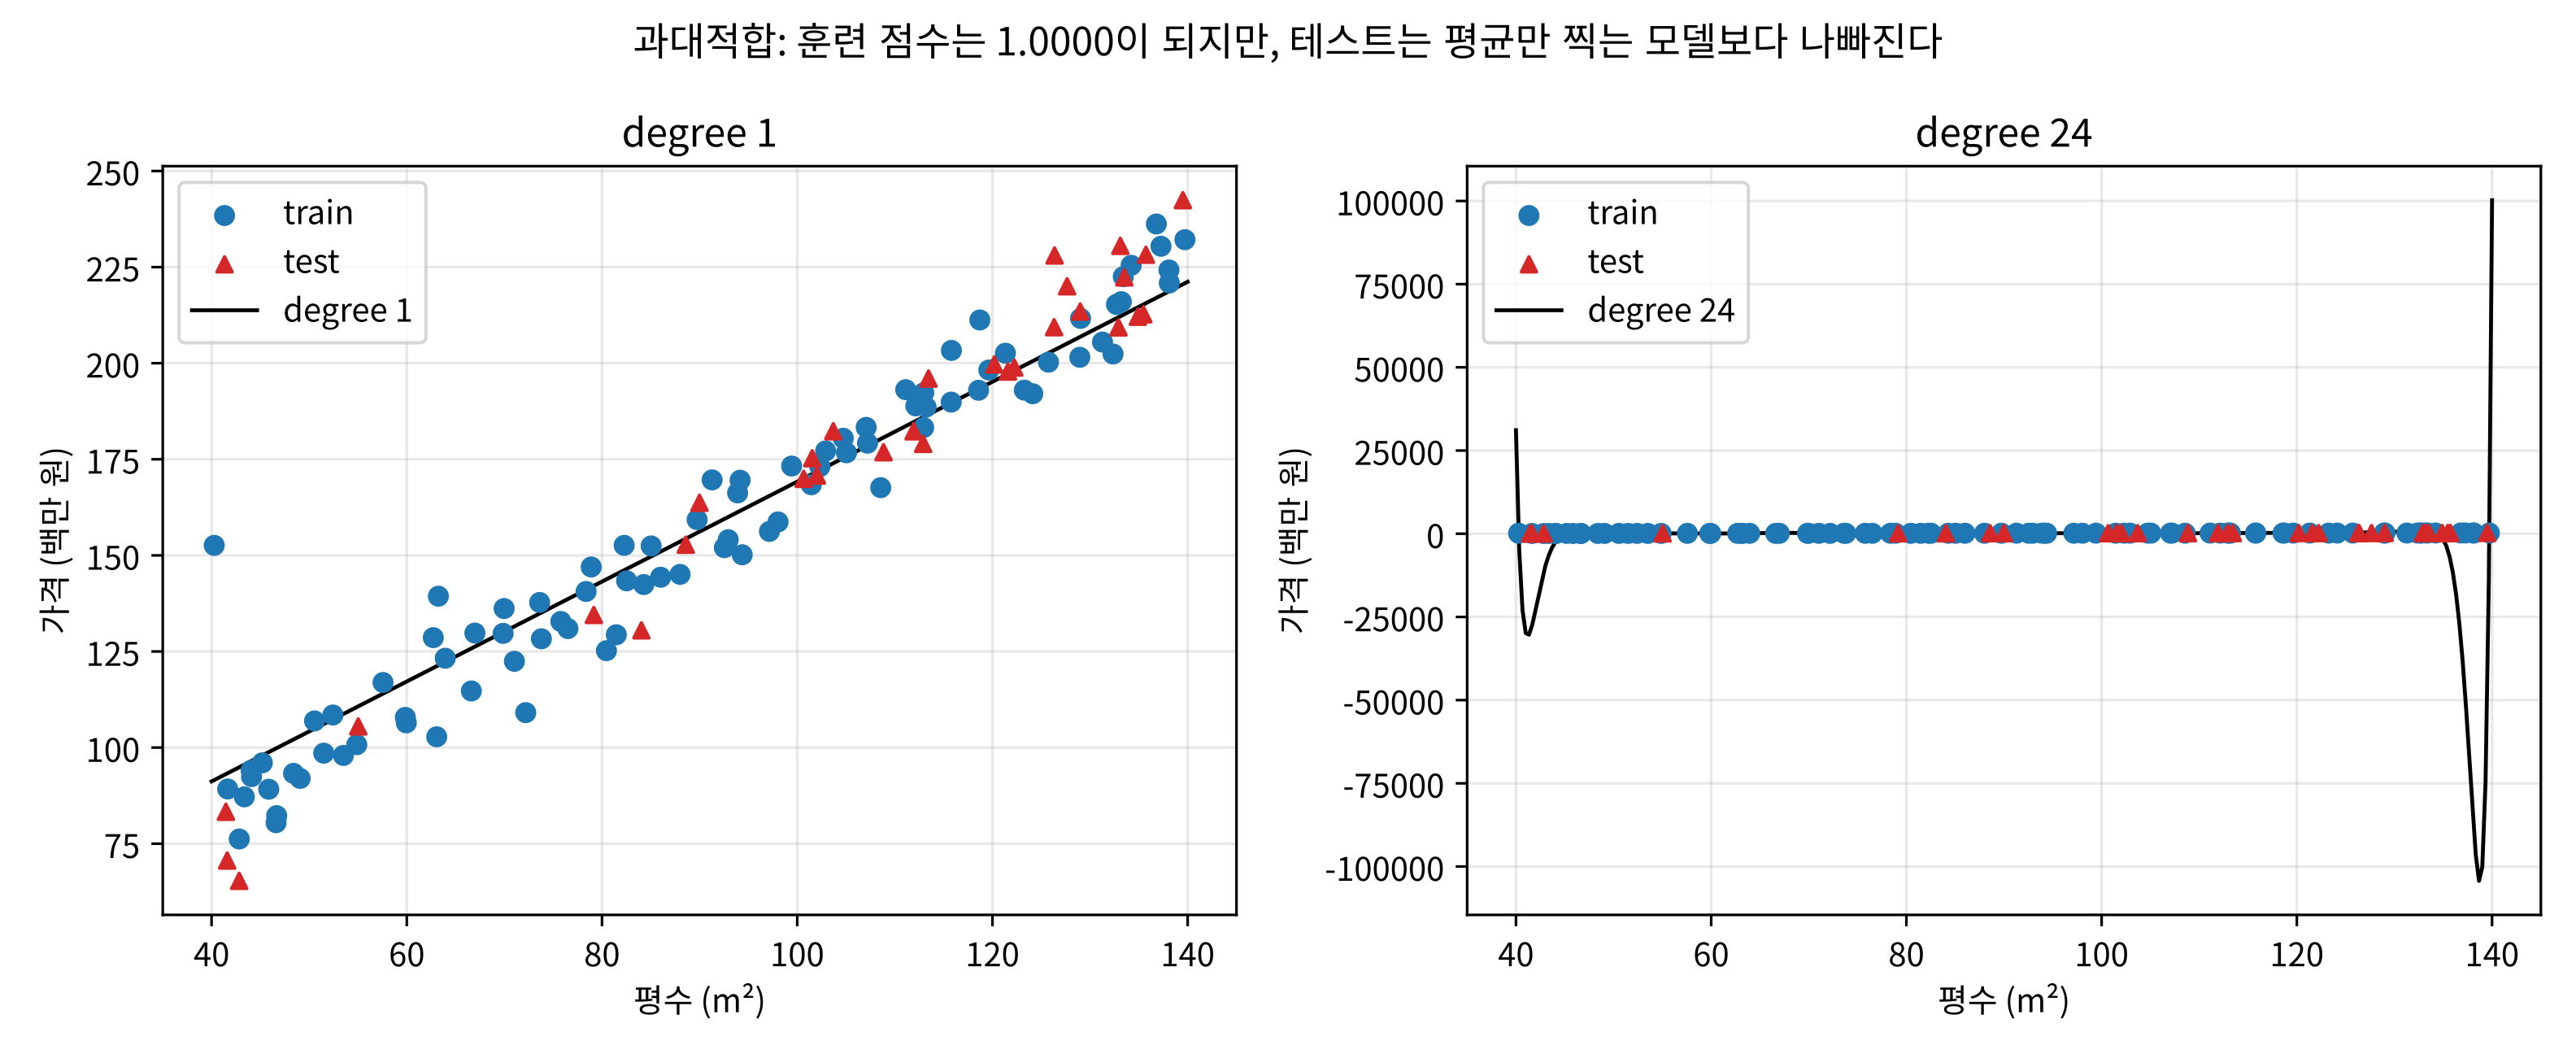
\includegraphics[width=\linewidth]{ch01_overfitting.png}
      \vskip0.4em
      {\footnotesize degree 1(왼쪽)은 점들의 경향에 따르는 한 줄,
      degree 24(오른쪽)은 25개 훈련 점(파랑)에 붙어 점과 점 사이
      잡음까지 외워 테스트(빨강)에서 광범위하게 흔들린다.}
    \end{column}
    \begin{column}{0.48\textwidth}
      \begin{itemize}
        \item 24차 다항식은 25개 훈련 점을 \textbf{완전히} 통과
          (train R²=1.0000 --- 매우 ``완벽''해 보임).
        \item 그런데 테스트 R²는 \textbf{마이너스 6만} ---
          ``평균만 예측하는 모델''(R²=0)보다 \textbf{몇만 배 나쁨}.
        \item 25개 파라미터가 25개 점에 정확히 맞춰지는 순간,
          다항식은 ``점들과 점들 사이에서'' 점에 붙어 있던
          \textbf{잡음 자체}를 외워버림.
      \end{itemize}
    \end{column}
  \end{columns}
  \vskip0.4em
  \begin{block}{핵심 교훈}
    \kq{``훈련 점수가 높다''는 사실은 잘 배웠다는 증거가 아니라,
    \textbf{외웠을 가능성}을 알리는 신호일 수 있으며, 모델이 좋은지
    나쁜지를 결정하는 것은 언제나 \textbf{보지 않은 데이터의
    점수}다.} (엄밀한 처리는 Ch.\,6.)
  \end{block}
\end{frame}

\begin{frame}{수학과 Python 사전지식 리뷰 --- 세 영역}
  이번 학기는 다음 세 영역의 수학을 \textbf{계속 재사용}한다 ---
  낯선 표기가 나올 때마다 이 절로 돌아와 확인할 것:
  \begin{itemize}
    \item \kb{선형대수}: 벡터의 \kb{내적}
      $w^\top x = \sum_j w_j x_j$, \textbf{행렬-벡터 곱}, 그리고
      \kb{그래디언트}(다변수 함수를 각 변수로 편미분해서 만든
      벡터, $\nabla_w J$). 고유벡터/고유값은 Ch.\,14(PCA)에서
      다시.
    \item \kb{미적분}: \kb{연쇄법칙 (chain rule)} --- 합성함수
      $f(g(x))$ 의 미분이 $f'(g(x))\,g'(x)$ 라는 것.
      \textbf{Ch.\,9(역전파)의 핵심 도구}가 바로 이것.
    \item \kb{확률}: \textbf{조건부 확률}과 \kb{베이즈 정리}
      \[P(y \mid x) = \frac{P(x \mid y)\,P(y)}{P(x)}\]
      Ch.\,3에서 본격적으로 사용.
  \end{itemize}
\end{frame}

\begin{frame}{손으로 한 번: 내적(4)과 연쇄법칙(42)}
  표기가 낯설다면 \textbf{아주 작은 숫자로 직접 계산}해보는 것이
  가장 빠르다.
  \begin{itemize}
    \item \kb{내적}: $w = [2, -1, 3]$, \; $x = [1, 4, 2]$ 일 때:
    \[w^\top x = (2)(1) + (-1)(4) + (3)(2) = 2 - 4 + 6 = 4\]
    \textbf{각 자리끼리 곱해서 다 더하는 것뿐} --- 이 계산이 이번
    학기 \textbf{거의 모든 챕터의 첫 줄}에 등장.
    \item \kb{연쇄법칙}: $g(x) = 3x+1$, \; $f(u) = u^2$, \; $x=2$
      일 때 $f(g(x)) = (3x+1)^2$ 의 미분:
    \[f'(g(x)) \cdot g'(x) = 2(3x+1) \cdot 3
      = 2{\cdot}7{\cdot}3 = 42\]
    직접 전개($(9x^2+6x+1$ 의 도함수 $18x+6$, \; $x=2$ 에서)해도
    \textbf{똑같이 42} --- 연쇄법칙은 ``안쪽을 미분하고 바깥쪽을
    미분해서 \textbf{곱한다}''는 지름길일 뿐, 다른 답을 주는 게
    아니다.
  \end{itemize}
  \vskip0.4em
  \begin{block}{두 가지를 기억하자}
    Ch.\,9에서 이 연쇄법칙 계산을 \textbf{한 번이 아니라 수십 개의
    층을 거쳐 반복}하게 된다 --- 지금 이 작은 예제가 그 전체 과정의
    \textbf{축소판}.
    실전에서는 numpy/PyTorch로 훨씬 빠르게 같은 계산을 하지만,
    처음 배울 때는 벡터 연산 뒤에 \textbf{숨은 for 루프를 직접 눈으로
    보는 쪽}이 이해에 더 도움이 된다는 판단에서, 개념 코드는 순수
    Python(리스트 + for 루프)으로 짠 경우가 많다.
  \end{block}
\end{frame}

\begin{frame}[fragile]{행렬-벡터 곱: numpy로 한 줄}
  \begin{lstlisting}
import numpy as np

X = np.array([[1.0, 2.0], [3.0, 4.0]])  # 2x2 행렬
w = np.array([0.5, -0.5])               # 길이 2 벡터
print(X @ w)   # 행렬-벡터 곱: [-0.5, -0.5]
\end{lstlisting}
  \vskip0.4em
  \begin{itemize}
    \item \texttt{X @ w}(행렬곱)는 앞으로 매 장에 나오는
      $w^\top x$ 형태의 계산을 \textbf{한 줄}로 표현 --- for 루프로
      직접 짜는 것보다 \textbf{빠르고 읽기 쉬움}.
    \item 이번 학기 수학의 전량은 \textbf{내적(4) + 연쇄법칙(42)} 이
      두 계산의 ``여러 번, 다른 형태로 반복''에 불과하다.
  \end{itemize}
\end{frame}

\begin{frame}{확인 문제: 파이프라인 원칙을 실제 상황에서 (a)(b)}
  \small
  \begin{itemize}
    \item \textbf{(a)} 이탈 라벨이 붙은 10,000행에서 EDA 결과
      ``이탈''이 \textbf{2\%뿐}. 이 사실이 파이프라인의 어느
      단계에 무엇을 바꾸는가?
    \item \textbf{답}: \kb{EDA의 발견이 평가 단계(지표 선택)를
      바꿈} --- 정확도는 ``전부 비이탈''로 예측해도 98\%라 이 문제
     에선 무의미에 가까움. \textbf{PR-AUC}(Ch.\,2.3) 같은 불균형
      클래스 지표를 처음부터 염두에 두고, 이후 단계(클래스
      가중, 샘플링 전략)를 계획.
  \end{itemize}
  \vskip0.4em
  \begin{itemize}
    \item \textbf{(b)} 1,000행에서 \texttt{age} 결측이 훈련부 10개,
      테스트부 3개. 평균으로 채운다 --- \textbf{어느 부분}의 평균을
      계산해야 하는가?
    \item \textbf{답}: \kb{훈련 부분} --- ``훈련에서 fit, 테스트에
      apply'' 원칙. 전체 평균을 쓰면 테스트 정보가 훈련에 살짝
      새는 형태.
  \end{itemize}
\end{frame}

\begin{frame}{확인 문제 (c)(d)}
  \small
  \begin{itemize}
    \item \textbf{(c)} 어떤 모델의 train R² = \textbf{0.99},
      test R² = \textbf{0.41}. 가장 가능성 높은 진단은? 24차
      다항식 예제와 어떻게 같은 이야기인가?
    \item \textbf{답}: \kb{과대적합} --- 모델이 훈련 데이터의 규칙
     이 아니라 \textbf{잡음을 외움}. 24차 예제(train R²=1.0000,
      test R²=$-$63495)가 이 현상의 \textbf{극단적 버전}. 두 경우
      모두 ``\textbf{훈련 점수가 높다}는 사실 자체''가 의심의
      대상.
  \end{itemize}
  \vskip0.4em
  \begin{itemize}
    \item \textbf{(d)} 새 데이터를 받아 실행 \textbf{전에}, 특징
      벡터가 완전히 같은 행 두 개가 \textbf{서로 다른 라벨}을 갖고
      있음을 발견. 가장 먼저 무엇을 해야 하는가?
    \item \textbf{답}: \kb{데이터 문제를 먼저 의심} --- Aha!
      데이터셋 사고가 정확히 이 상황.
      \texttt{df.duplicated(keep=False)} 로 몇 개인지 파악한 뒤,
      하나를 제거할지 라벨을 재확인할지를 \textbf{도메인 지식을
      바탕으로} 결정 (알고리즘을 바꾸는 문제가 아님).
  \end{itemize}
\end{frame}

\begin{frame}{1.3 마무리}
  \begin{block}{한 줄 요약}
    \kq{모델은 파이프라인 다섯 단계 중 하나일 뿐 --- 그리고
    모델의 상한을 가장 결정적으로 좌우하는 단계는 모델이 아니라,
    ``데이터가 얼마나 깨끗하고 충분히 이해되었는가''다.}
  \end{block}
  \vskip0.6em
  \begin{itemize}
    \item 파이프라인: \textbf{수집 $\to$ 정제 $\to$ EDA $\to$
      모델링 $\to$ 평가} --- 결함은 위에서 아래로 \textbf{증폭}.
    \item train/test는 \textbf{나누기 전에} 통계량을 계산하면
      \textbf{누수} --- ``훈련에서 fit, 테스트에 apply''.
    \item 수학 전량은 \textbf{내적(4) + 연쇄법칙(42) + 베이즈
      정리} --- 낯선 표기가 나올 때마다 이 절로.
  \end{itemize}
\end{frame}

% ===== 이번 주차 정리 =====
\begin{frame}{이번 주차 정리}
  \small
  \begin{enumerate}
    \item \kb{1.1 역사와 로드맵}
      \begin{itemize}
        \item 역사는 직선이 아님 --- \textbf{두 번의 AI 겨울}(1969 XOR
          증명, 1986 역전파로 해소)과 2012 AlexNet.
        \item 돌파구의 반복 패턴: \textbf{새 수학이 아니라 데이터+
          계산의 재조합}. Block A(Ch.\,2$\sim$7 고전 ML) $\to$
          Block B(Ch.\,9$\sim$16 신경망$\to$생성모델).
      \end{itemize}
    \item \kb{1.2 문제 정식화와 세 갈래}
      \begin{itemize}
        \item 알고리즘보다 먼저: \textbf{$x$ · $y$ · $h$ 로 정의}.
          ``라벨이 있는가? 보상이 있는가?'' 두 질문으로
          \textbf{지도/비지도/강화}를 가름.
        \item 회귀 vs 분류 = \textbf{같은 모델, 다른 출력}(항등 vs
          시그모이드 링크) · 모든 알고리즘의 뼈대 =
          \textbf{$J$ 정의 $\to$ 최소화}.
      \end{itemize}
    \item \kb{1.3 파이프라인과 사전지식}
      \begin{itemize}
        \item 모델링은 5단계 중 하나 --- 더티 데이터(결측·중복·
          이상치)·EDA·\textbf{train/test 순서(누수 방지)}가 모델의
          상한을 결정.
        \item 수학 전량 = \textbf{내적 · 연쇄법칙 · 베이즈 정리}.
      \end{itemize}
  \end{enumerate}
  \vskip0.6em
  \begin{block}{다음 주차 --- Chapter 2. 회귀 모델: 선형회귀와
  로지스틱회귀}
    이 책의 첫 번째 모델. 그 도입부에는 이미 19세기 수학자가 잡음
    섞인 점들 사이를 ``모두를 가장 잘 맞혀주는'' 한 줄로 통과시켜야
    할 문제가 등장한다 --- 오늘 세운 ``\textbf{손실함수를 정의하고
    최소화한다}''는 틀과 \textbf{내적·그래디언트 감각}이 있으면,
    그 문제는 낯선 수학이 아니라 바로 이 챕터의 \textbf{연장선}으로
    읽힌다.
  \end{block}
\end{frame}

\end{document}
